\documentclass[10pt,a4paper]{article}
\usepackage[svgnames]{xcolor}
\usepackage{pdftexcmds}
\usepackage[utf8]{inputenc}
\usepackage{amsmath}
\usepackage{amsfonts}
\usepackage{tikz}
\usepackage[tikz]{bclogo}
\usetikzlibrary{shapes,arrows,automata,fit}
\usepackage{amssymb}
\usepackage{graphicx}
\usepackage{wrapfig}
\usepackage{helvet}
\usepackage{pgf-umlsd}
\usepackage{textcomp}
\usepackage{minted}
\author{Gokudomatic}
\title{Tutorial for a kinematic FPS game}
\date{\today\\v1.0}
\renewcommand{\familydefault}{\sfdefault}

\tikzstyle{node} = [draw, fill=blue!20, text centered, rounded corners]
\tikzstyle{decision} = [diamond, draw, fill=blue!20, 
    text width=4.5em, text badly centered, node distance=3cm, inner sep=0pt]
\tikzstyle{block} = [rectangle, draw, fill=blue!20, 
    text width=5em, text centered, rounded corners, minimum height=4em]
\tikzstyle{line} = [draw, -latex']
\tikzstyle{cloud} = [draw, ellipse,fill=red!20, node distance=3cm,
    minimum height=2em]

\tikzset{
  line/.style ={draw, thick, -latex', shorten >=0pt}
}

\newcounter{tutorialStep}

\newcommand{\step}{%
  ~\\\\\stepcounter{tutorialStep}%
  \Large\textcolor{blue}{\arabic{tutorialStep}) }\normalsize}

\newminted{python}{frame=single,gobble=2}

\newenvironment{warning}{%
  \begin{bclogo}[logo=\bcattention, couleurBarre=red, noborder=true, 
               couleur=LightSalmon]{Important!}
}{%
  \end{bclogo}\hspace{1px}\\
}

\newenvironment{hint}{%
\begin{bclogo}[logo=\bcinfo, couleurBarre=Green, noborder=true, 
               couleur=white]{Hint}
}{%
\end{bclogo}\hspace{1px}\\
}

\begin{document}

\maketitle

\clearpage

\begin{center}
{\Large Revisions}
\begin{tabbing}
\hspace{1cm} \= \kill
1.0 \> Original draft
\end{tabbing}
\end{center}

\clearpage

\tableofcontents

\clearpage

\section{Introduction}

\subsection{Preface}
Hi folks! 
Today we're going to build a basic FPS (First Person Shooter) game with Godot. The highlights of this tutorial are setting up a 3d project, importing 3d models and implement a script to make the character move like in old FPS games like Doom\cite{doom}, Duke Nukem or Half Life.\\
\\
I decided to write this tutorial when I was working on another Godot project which requires characters able to move in a 3d world. I noticed that Godot was not offering out of the box such features and the existing similar demos (3d platformer, kinematic char and FPS Test) do not provide exactly a ready to use solution that behaves like in the games mentioned above. I played then for a while, trying to understand little by little the code of the existing demos and figure out why they behave strangely in some situations, like slopes and stairs. Finally I got a satisfying implementation of a solution using kinematics and a couple of others concepts. And then I decided to share this work in the shape of a tutorial. I hope it will at the same time help beginners to understand how to build a 3d game with self made assets.\\
It won't cover however the basic stuffs from Godot, like the concept of nodes, the scripting language GDScript or the user interface. If you are interested in those topics, I wrote a 2d demo\cite{fox2d} with a documentation that explain how nodes work in Godot and their capabilities.\\
\\
I'm aware that as any tutorial, this one will eventually become outdated. However I'll try as much as possible to explain the maths behind, which is the most important part of this tutorial. I hope that even if Godot changes radically, you can still be able to rewrite easily the code. In fact, if you can even implement it in another game engine (Unity for instance), this document reached its objective.

\paragraph{What it covers} 
Within this tutorial, you'll learn to:
\begin{itemize}
\item Create a 3d scene.
\item Prepare a 3d model in Blender and export it.
\item Import 3d models in Godot.
\item Implement a kinematic based First Person View character.
\item Create lifts and ladders.
\item Create actionable doors and buttons.
\end{itemize}

\paragraph{What it doesn't cover}
This tutorial does not intend to explain every part of an FPS game, as it would be too much to explain in one tutorial. And that would be too specific to one kind of gameplay anyway. What won't be covered, among lot of others stuffs, are:
\begin{itemize}
\item Sounds
\item Lights and shadows
\item Enemies, NPC and bullets
\item HUD and menu
\item Death by falling or being crushed
\item How to make a 3d model. I briefly cover how to build a map in inkscape and blender, but I assume you know how to use those softwares. It will mostly be hints and tips specific to godot.
\end{itemize}

\subsection{Target audience}
This document is destined to advanced beginners. A basic knowledge in Godot (IDE, nodes, script language) and in programming, including UML, is mandatory to properly understand this tutorial. \\
Knowledge in Sketchup and Blender is also helpful, but you can download the 3d model from the project if you want to skip the modelling part.
\paragraph{About math} a good understanding of vectors is required. It is advised to get a grasp of the basics of quaternions too since we're going to use them a bit. You can find tutorials about those points in the wiki of Godot \cite{wiki_godot}.

\subsection{Requirements}
For this tutorial, you need to install:
\begin{itemize}
\item Godot v1.0 or later \cite{godot}
\item Blender 2.7 or later \cite{blender}
\item Better Collada exporter plugin for Blender provided with Godot. You'll have to install it in the Blender folder.
\end{itemize}
I will also use Sketchup \cite{sketchup} and textures from Freedoom\cite{freedoom}, but it is optional. If you use Sketchup, you'll need a script\cite{sketchup_stl} to export your model to STL format.\\
\\
This tutorial was written in Xubuntu 14.10 with a night build from Godot and Blender 2.72b, as well as Sketchup 8 through Wine. The Better Collada exporter is however from the stable version 1.0 of Godot, since the night build version when I was writing this document had a bug.

\subsection{How to read}
This document should be read step by step. If you don't want to use sketchup, you can skip chapter \ref{sec:sketchup}. And if you have already a collada map or if you want to use the map of this tutorial, you can also skip chapter \ref{sec:blender}.

\subsection{Terminology}
The steps of the tutorial are displayed like this:
\step Step one
\step Step two
\step Step three\\
\\
GDScripting code:
\begin{pythoncode}
  # comment
  var v=Vector3(1,0.5,10)
  print("vector: ",v)
  func _process(delta):
    pass
\end{pythoncode}
References to source code(variables, node names, classes) or Godot API are in \textit{italic}.\\
\\
Files, folders and paths are "quoted". The paths will always be relative paths.\\
\\
Warnings and important information:
\begin{warning}
    This is an important note.
\end{warning}
Hints and tips:
\begin{hint}
    This is a tip.
\end{hint}
Keyboard hot-keys will be displayed like this : \textbf{[Ctrl-A]}\\
If, like often in Blender, a sequence of keys must be pressed, it will be displayed like this : \textbf{[A,B,C,D]}

\subsection{About the author}
I'm essentially a programmer with a few experience in 2d and 3d graphics. I have some personal experience in game programming, mostly in Java and Delphi, yet all my projects were for personal training and didn't reach any public status.\\
I played with Godot almost since it was open-sourced, but because my knowledge in 3d math are weak, I was mostly sticking with the 2d part of the engine.

\setcounter{tutorialStep}{0}

\section{Project folder structure}
Let's start!
\step Create a folder with 2 subfolders named "assets" and "source".
\begin{hint}
The folder "assets" is for all your media files. In this case, it will be sketchup and blender files, as well as textures. But it would be for audio files too if your game uses some, which is most probably the case.\\
The folder "source" the Godot project itself and all its source code.\\
By separating the assets and source, you won't distribute the original files of your assets when you export your project.
\end{hint}
\step Open Godot and create a new project in the folder "source".
\step In the "source" folder, create a folder named "game\_assets".
\begin{hint}
This subfolder will containt all assets that need to be distributed with the game. 
\end{hint}
\step Copy all the textures you need in both "assets" and "game\_assets" folders.
\begin{hint}
For big projects, it is strongly recommended to use a VCS (Version Control System) for at least the "source" folder.
\end{hint}


\paragraph{Note} As a general rule, save regularly. No matter which tool you're using, don't forget to save in case of a crash.

\section{Build the map in Sketchup}
We're going here to draw everything specific to the map, including elevators and ladders. You are free to draw any kind of map, but to properly show what the demo can do, it's better that it includes at least:
\begin{itemize}
\item 1 elevator
\item 1 button
\item 1 ladder
\item 1 slope of 30° or less (where you can stand on)
\item 1 slope steeper than 45° (where you'll slide)
\end{itemize}
I'll add a door later in Blender because it is more convenient.

\begin{hint}
Elevators, buttons and others non-static objects can be drawn here. But for larger projects, you might prefer to make reusable models, since buttons and doors need script. In this case, it is better to add them later in Godot.
\end{hint}

\label{sec:sketchup}
\subsection{Draw the map}
\step Open a new project in Sketchup and set the view on top. Then draw the rooms. (1) is the player initial position, and (2) is the goal to reach.\\
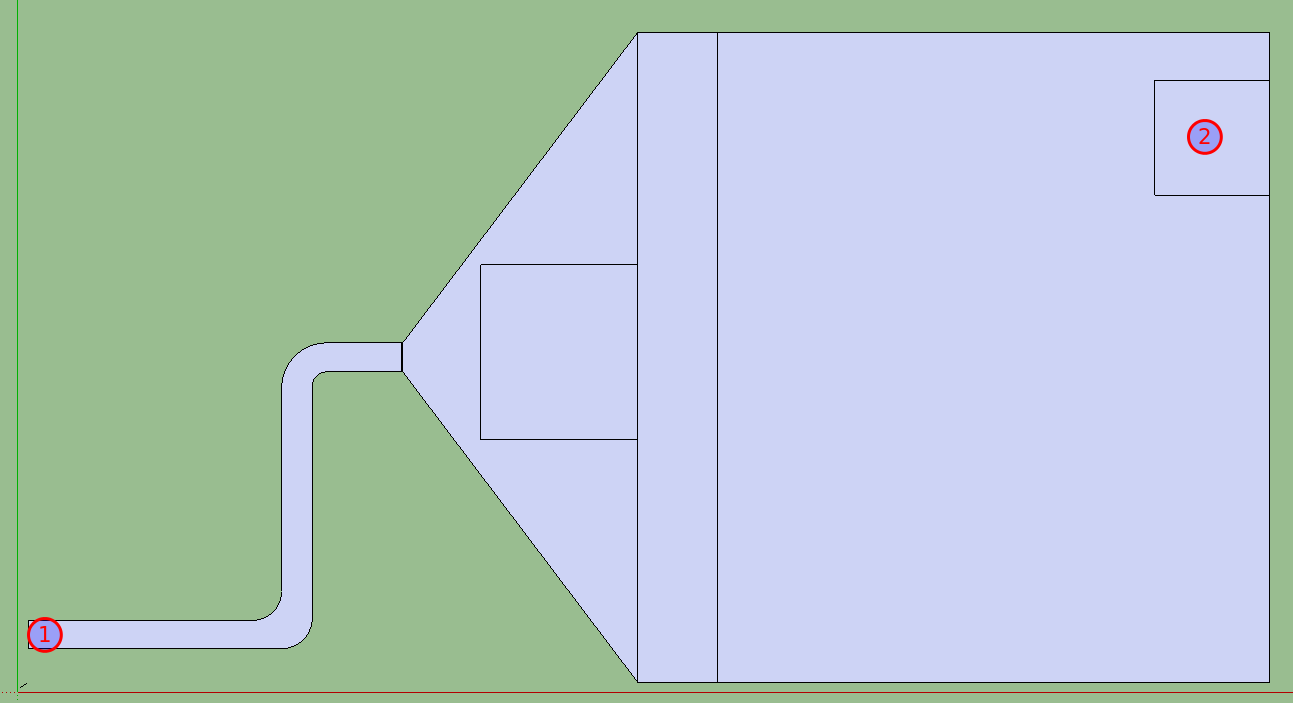
\includegraphics[scale=0.3]{map_step1.png} 
\step Extrude the rooms to make walls and ceilings.
\step Create stairs (1), extrude from the wall a platform for the goal (2), and make a ladder (3).\\
 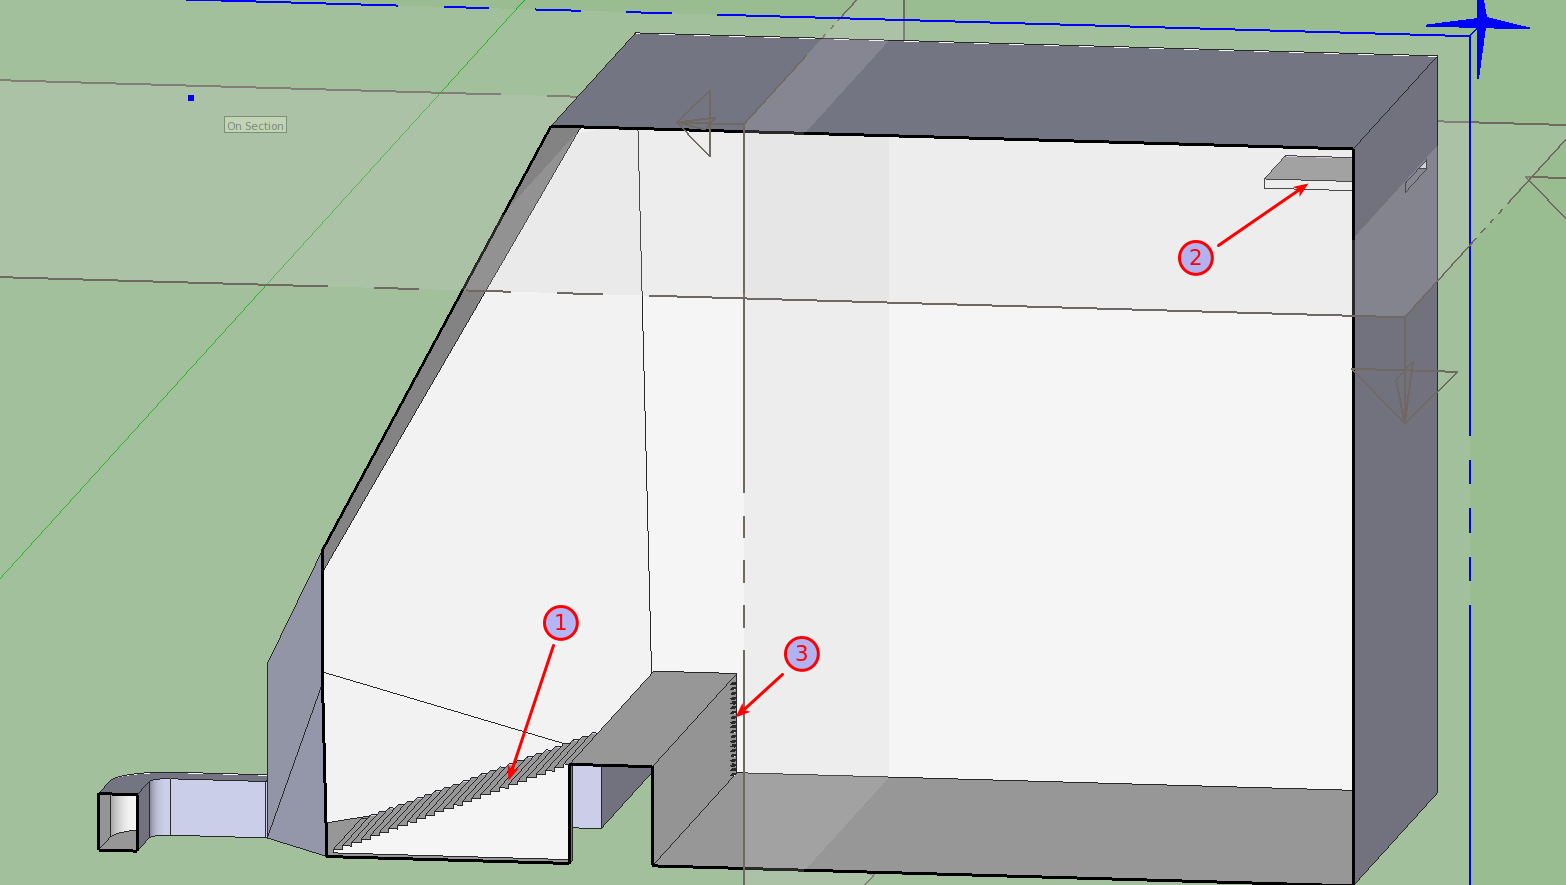
\includegraphics[scale=0.25]{map_step2.png} 
\step The ladder can have any shape you whishes. It just need to be vertical.\\
 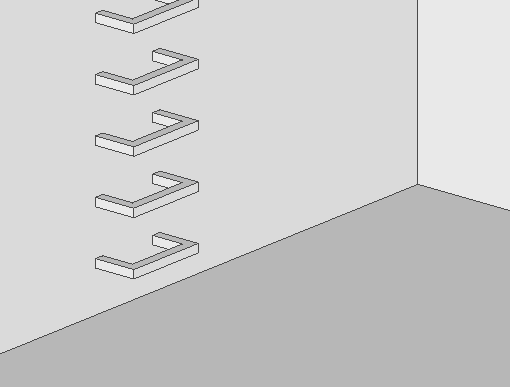
\includegraphics[scale=0.75]{map_step3.png} 
\step Create 2 blocs in the middle of the room (1) \& (2), and a bridge between them with a slope of 30°. And finally make a platform (4) that will be an elevator between the bloc (2) and the goal.\\
 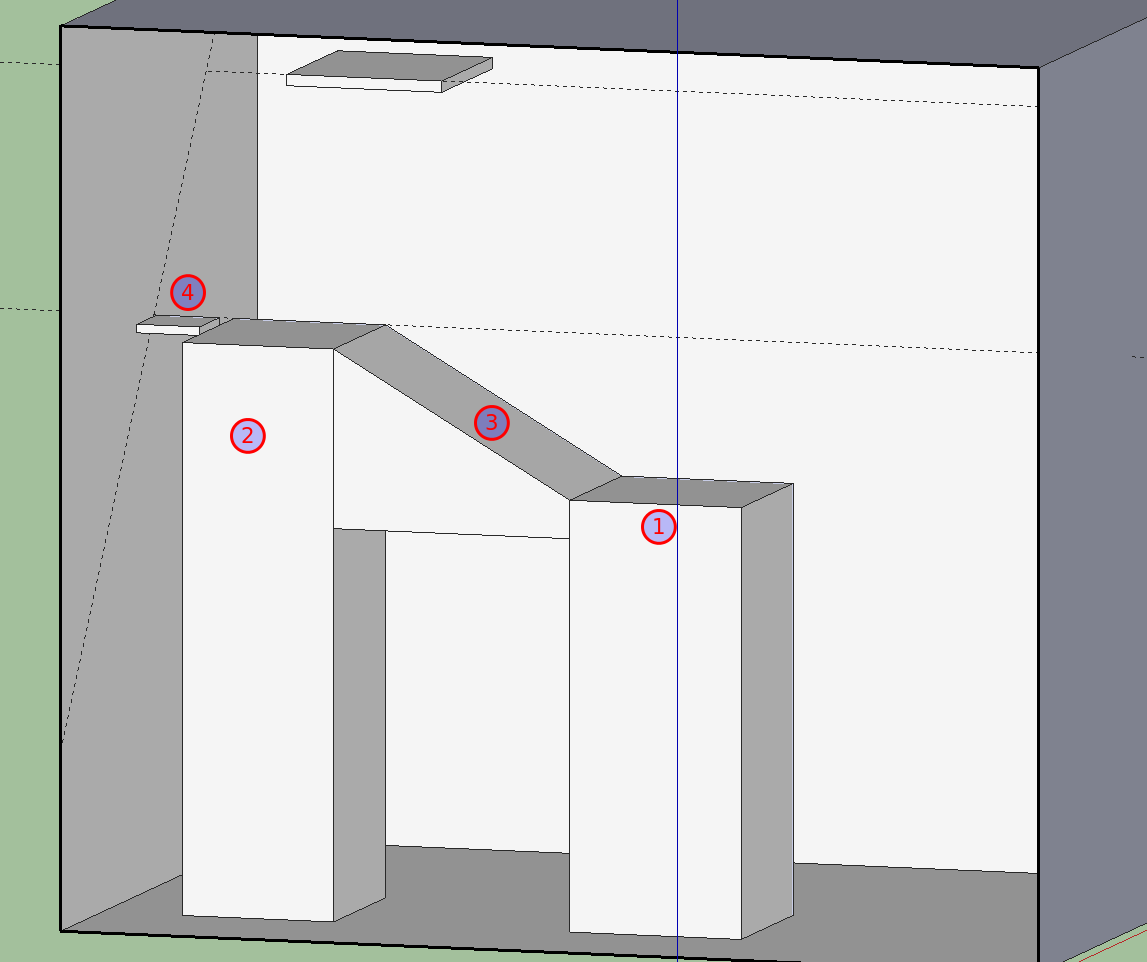
\includegraphics[scale=0.3]{map_step4.png} 
\step Draw another platform that will travel between (1) and (2).\\
 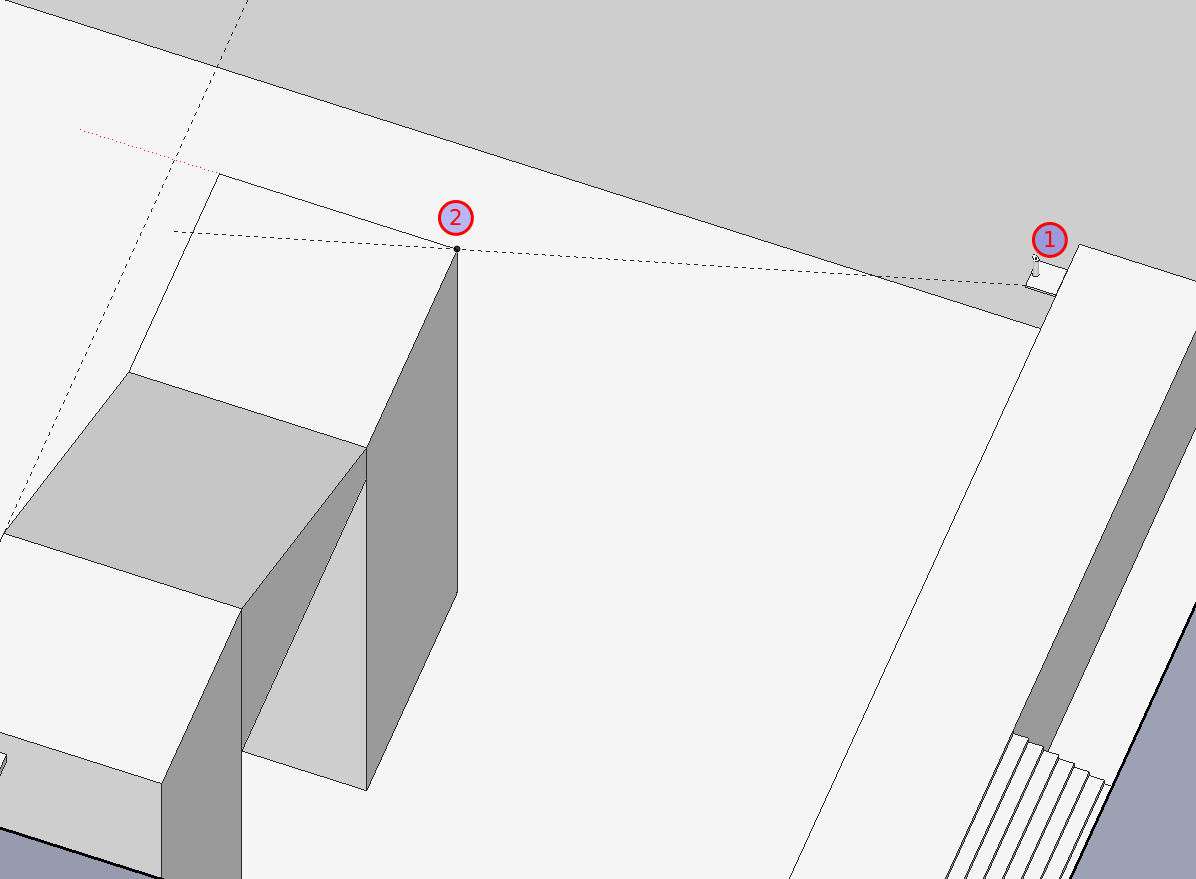
\includegraphics[scale=0.3]{map_step5.png} 
\step On this platform draw a button that will activate the platform/elevator.\\
 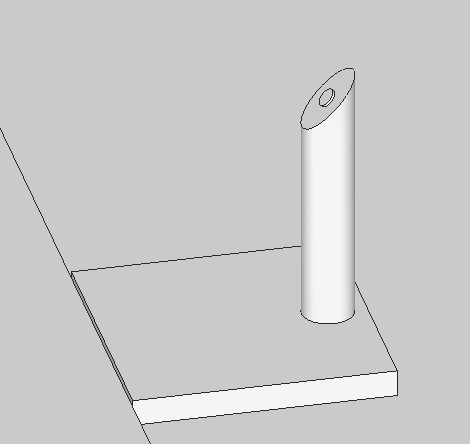
\includegraphics[scale=0.7]{map_step6.png} 
\step Make a bridge(1) between the platform of the goal and the second bloc. This bridge must have a steep slope ( \textgreater 45°).\\
 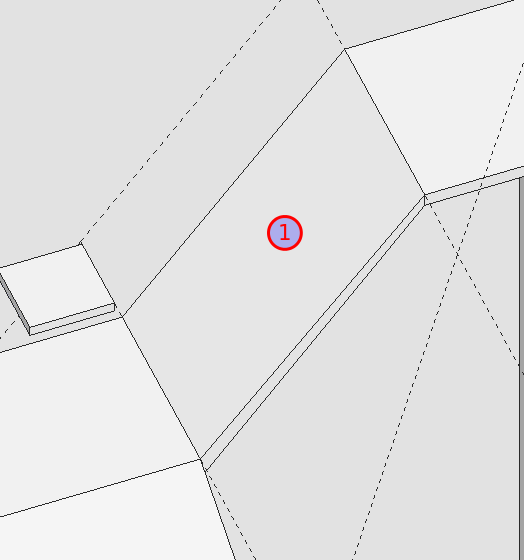
\includegraphics[scale=0.6]{map_step7.png} 
\step Be sure to remove all construction lines.

\begin{hint}
No need to add textures here, since the export doesn't include them.
\end{hint}
\begin{hint}
Sketchup gives by default a little character and a unit for dimensions. You can use them to estimate appropriate dimensions for your building. Personally I use the meter unit. It is possibly anyway to resize it later.
\end{hint}
\begin{hint}
When you draw round shapes, expect Sketchup to make lot of faces, since the whole mesh will be converted to triangles. It will be easier to work with the mesh if those areas are small. With the pencil tool, you can draw edges to help the exporter making cleaner faces.\\
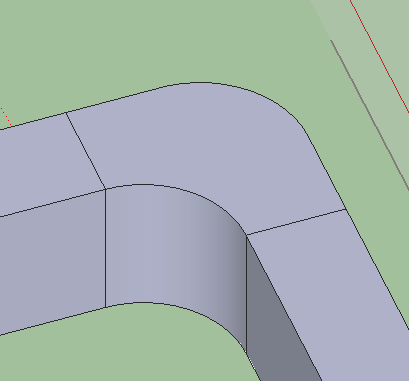
\includegraphics[scale=0.5]{map_sketchup_hint_faces.png} 
\end{hint}
\subsection{Export to STL}
\begin{warning}
Delete or disable all section planes, since only what's visible is exported.
\end{warning}

\step Be sure nothing is selected and go in menu Tools / Export to DXF or STL \\
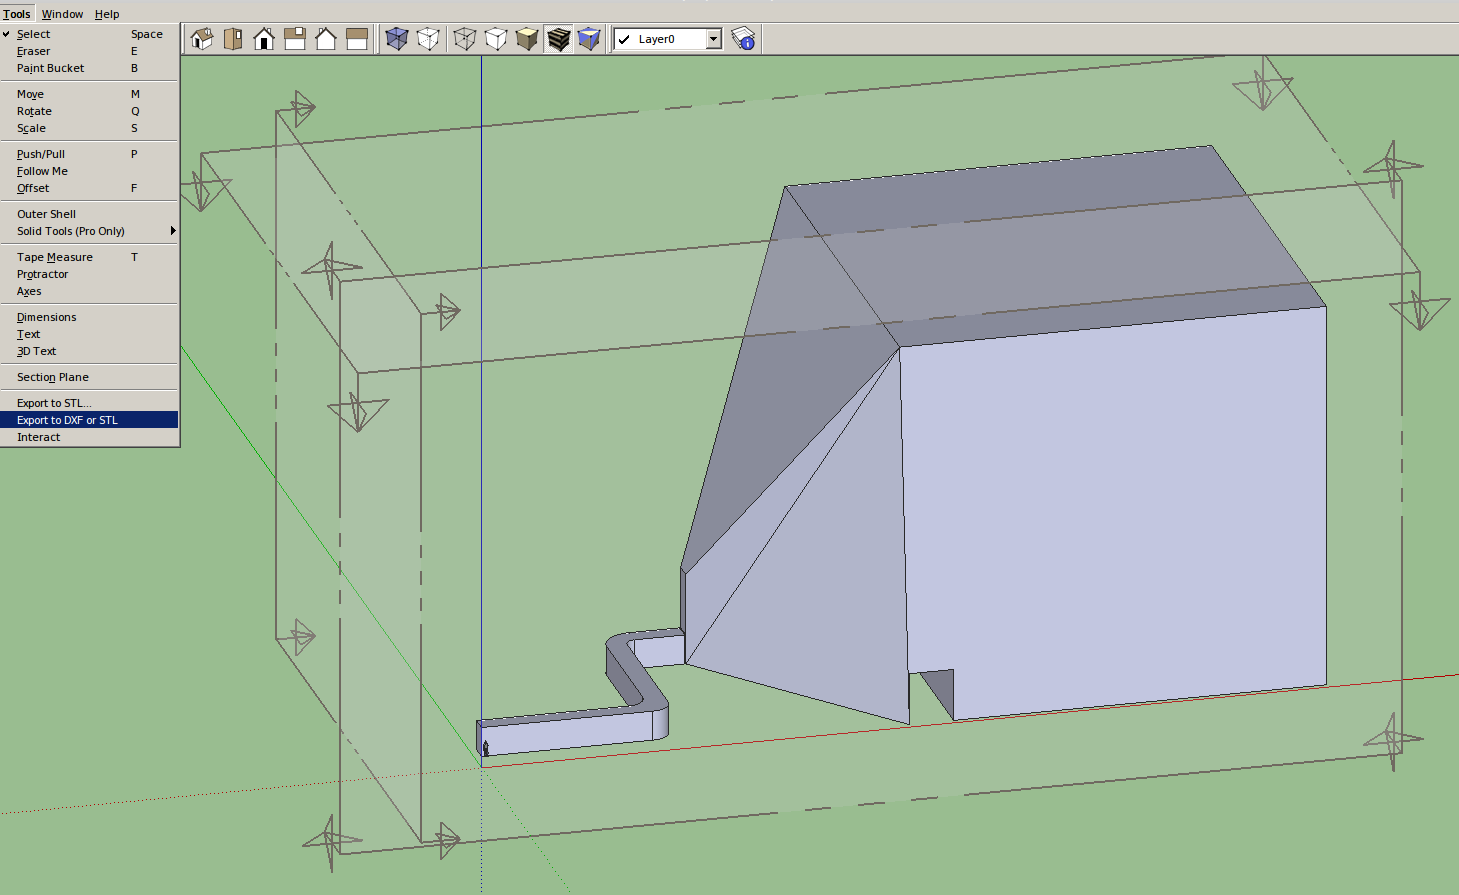
\includegraphics[scale=0.25]{export_stl_step1.png} 
\step Accept to export entire model\\
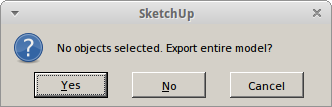
\includegraphics[scale=1]{export_stl_step2.png} 
\step Choose Meter unit\\
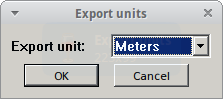
\includegraphics[scale=1]{export_stl_step3.png} 
\step Choose stl\\
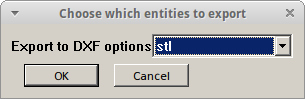
\includegraphics[scale=1]{export_stl_step4.png} 
\step Save to "map.stl" in the "assets" folder\\
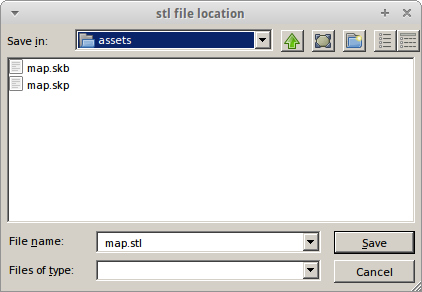
\includegraphics[scale=0.8]{export_stl_step5.png} 

Now the map is exported to STL format and can be imported in Blender.

\section{Prepare the map in Blender}
\label{sec:blender}
\subsection{Import STL}
\step Start Blender
\step Remove everything \textbf{[I,I,X]}
\step Import the STL file (menu File / Import / Stl). Use the default options.
\begin{hint}
If the STL importer is not in the list, check that the STL format plugin is enabled in the User Preferences / Addons.
\end{hint}
\step You should now see your map.\\
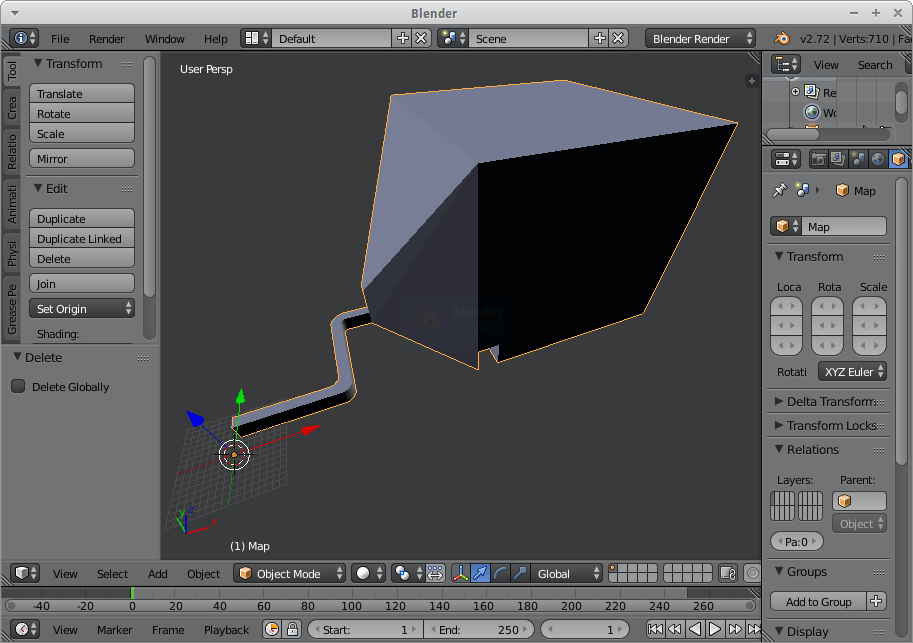
\includegraphics[scale=0.4]{blender_step1.png} 
\step Save the file in the same folder. \textbf{[Ctrl-S]}
\subsection{Normals}
We must now check that all face normals are properly oriented inward.
\step Select the mesh
\step Enter in edit mode \textbf{[Tab]}
\step Open the properties panel \textbf{[N]}
\step Look for Mesh Display and activate the Display face normals as line. Set the size to something visible, like 5. The normals should show up as cyan lines.\\
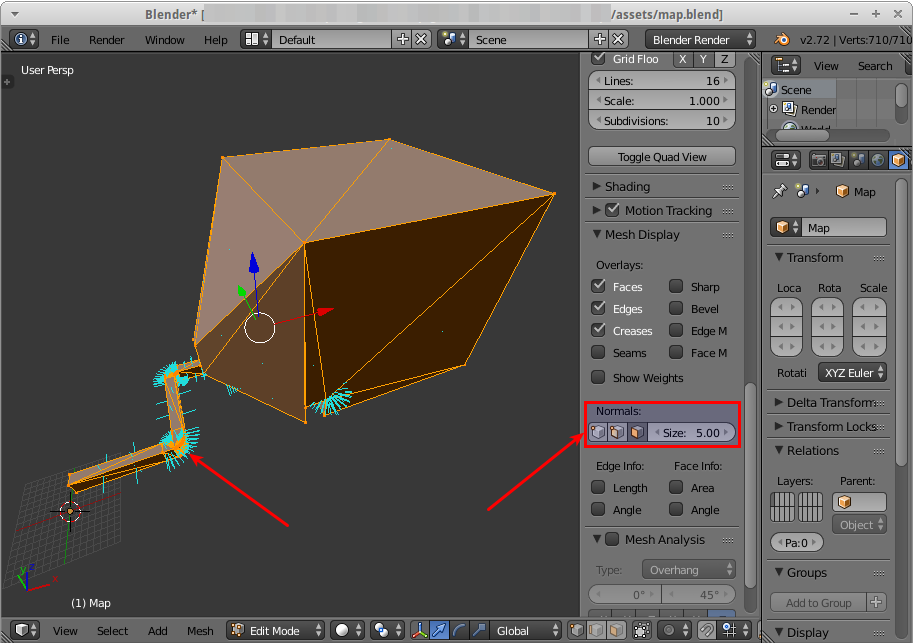
\includegraphics[scale=0.4]{blender_step2.png} 
\step Reduce the size of the normal, like back to 0.1, and check that no normal is pointing outside. You should see only dots.\\
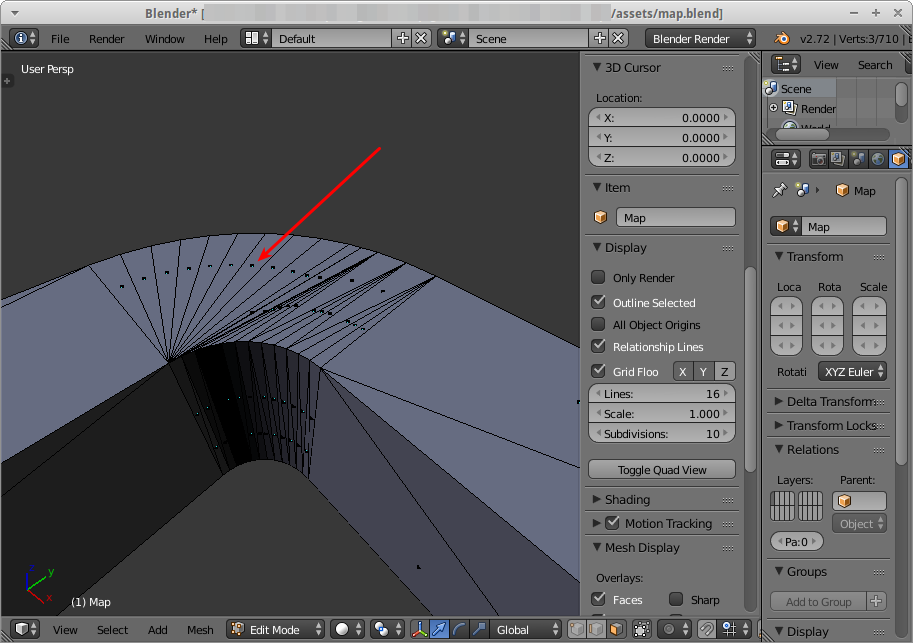
\includegraphics[scale=0.4]{blender_step3.png} \\
\begin{hint}
If you find a face with the normal pointing outside, you can invert it with menu Mesh / Faces / Flip Normals. \textbf{[Ctrl-F,F]}.
\end{hint}
\step At the same time, you can remove unwanted faces or vertex.\\
\begin{hint}
You can hide faces with \textbf{[H]}, and show all hidden faces with \textbf{[alt-H]}.
\end{hint}
\step Disable the display normal when you're done.
\subsection{Separate elevators}
The elevators made in Sketchup are actually part of the map. But in Godot they need to be separate meshes.
\step In edit mode, select all vertices of one elevator and separate it with \textbf{[P,1]}.\\
\begin{hint}
You can easily select all vertices by selecting one and select all linked vertices \textbf{[Ctrl-L]}.
\end{hint}
\step Repeat the previous action for for each elevator.
\subsection{Textures \& UV mapping}
\step Go back to object mode \textbf{[Tab]} and open the UV/image editor.
\step Open each texture from the "assets" folder to load them in memory.
\step Go back to the 3D View, select the map mesh and go in edit mode \textbf{[Tab]}.
\begin{hint}
For conveniency split the view in 2 and keep visible both 3D View and image editor.\\
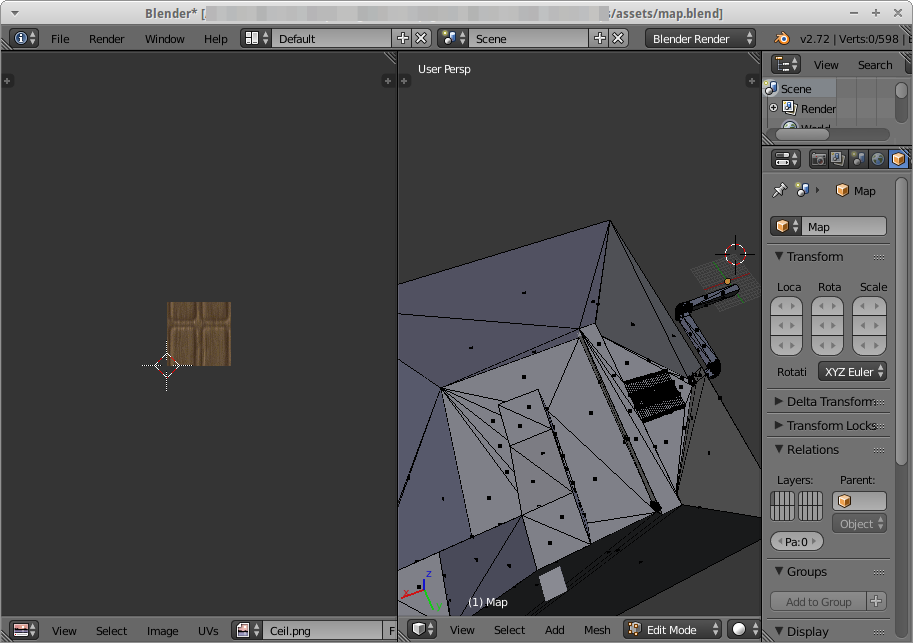
\includegraphics[scale=0.4]{blender_hint_split_panels.png} 
\end{hint}
\step Select all faces that are the same kind, for instance the floor. They will have the same texture.
\step In the Properties view, select the Material Tab.\\
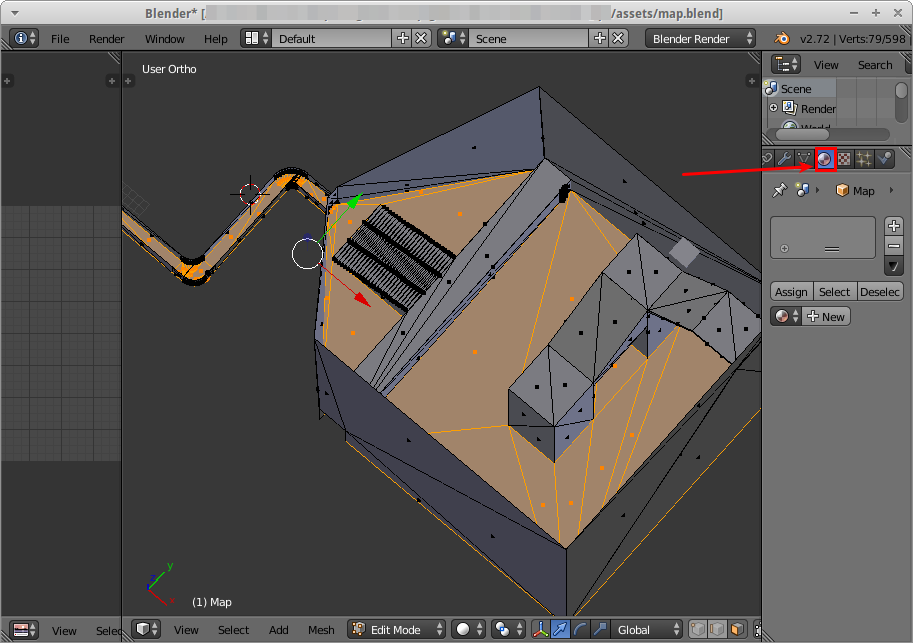
\includegraphics[scale=0.4]{blender_step4.png} 
\step Create 2 material slots (1) and a new material for each.
\step Select the second material slot (2) and click "Assign" (3) to assign the currently selected vertices to the material.\\
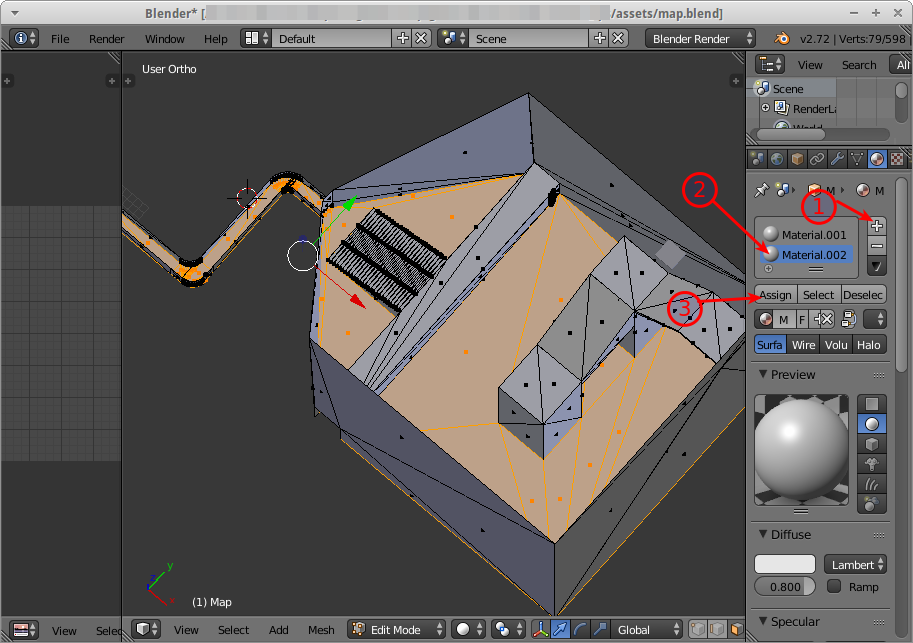
\includegraphics[scale=0.4]{blender_step5.png} 
\step Rename the first material slot as "Wall" and the second material slot as "Floor1".
\begin{hint}
The first material slot created is by default assigned to the whole mesh. That's why I selected the second material slot to assign the vertices.
\end{hint}
\step Create as many new material slot as there are textures, except for the two already created. And assign the vertices that should be linked with the texture. In my case, I have 1 wall texture, 1 ceiling texture and 2 floor textures. I had to create 2 others slots for the ceiling and the other floor textures. On top of that I created a special material slot for the ladder, without texture but with a gray color.
\step Repeat the same actions for the elevators. You can however reuse existing materials. I had still to create a new material for the button, which I wanted red.
\step For the button material and the ladder material, set some colors.\\
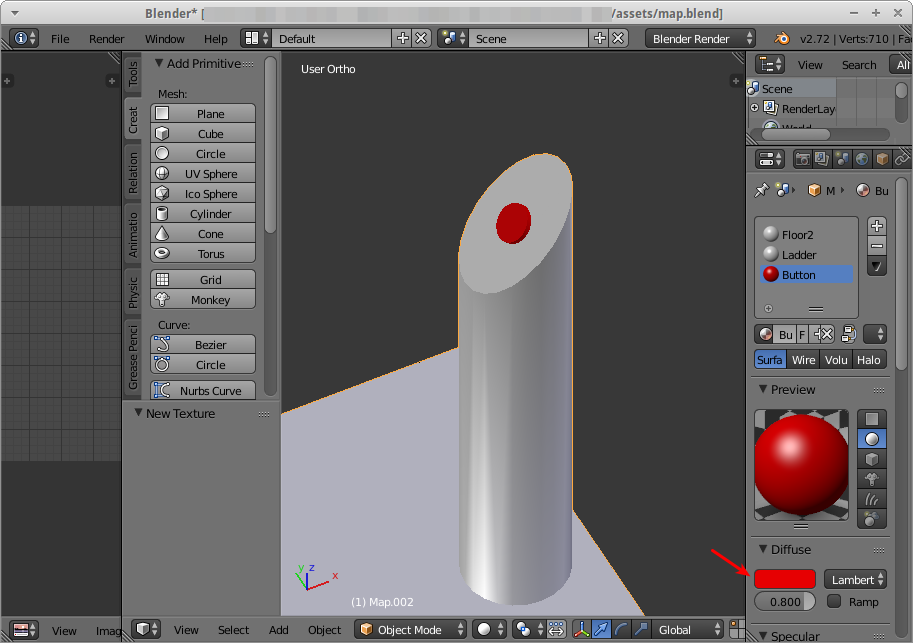
\includegraphics[scale=0.4]{blender_step6.png} 
\step Now, we'll apply some texture. Select the material slot that will have a texture (1) and click "select" (2) to select all associates vertices.
\step Go in the Texture tab (3)\\
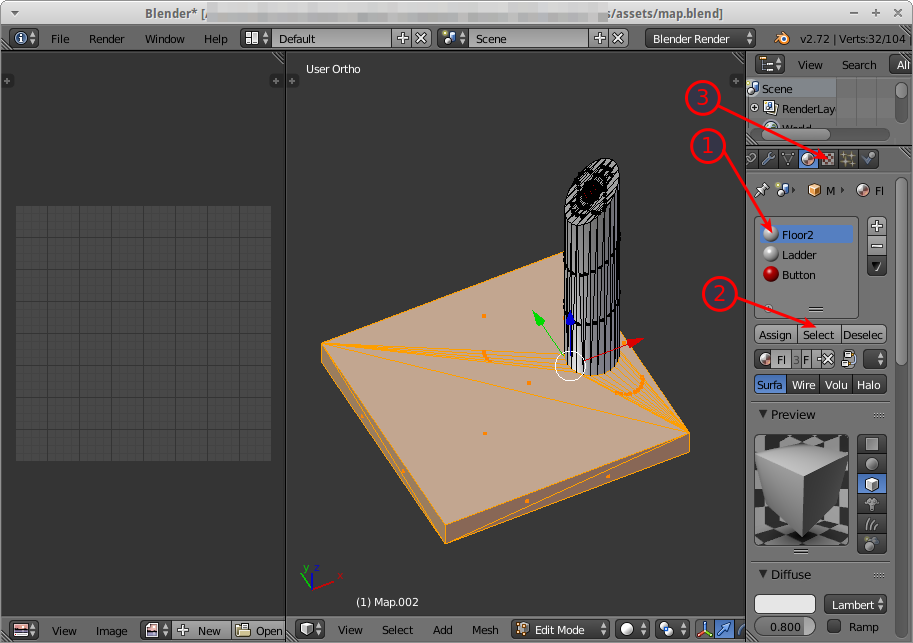
\includegraphics[scale=0.4]{blender_step7.png}
\step Create a new texture\\
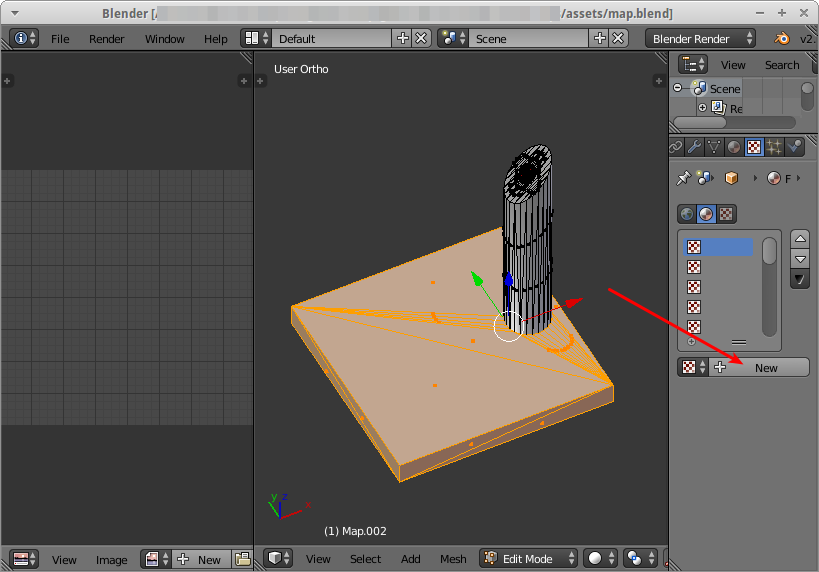
\includegraphics[scale=0.4]{blender_step8.png}
\step Open the list of loaded images (1) and choose the appropriate image (2)\\
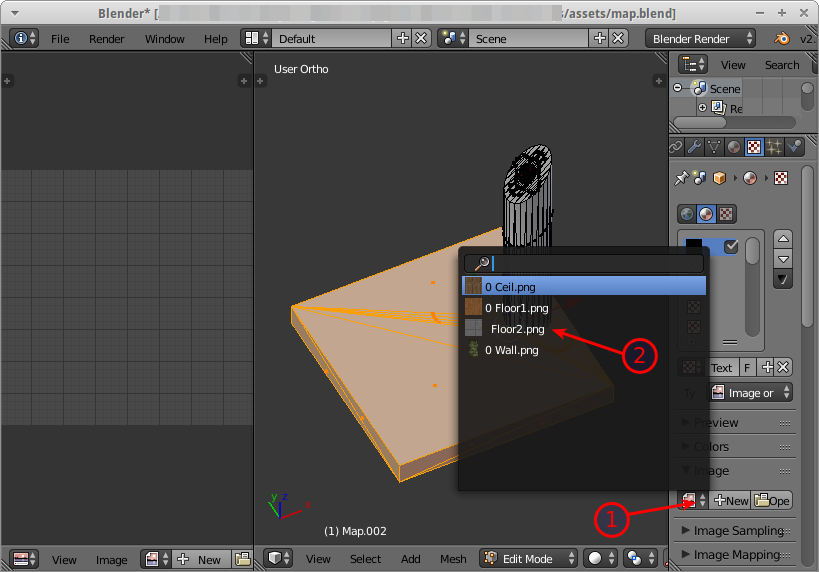
\includegraphics[scale=0.4]{blender_step9.png}
\step In the image editor, select the same image (1). With the mouse, go in the 3D view and open the unwrap menu \textbf{[U]}. Choose "Cube Projection".\\
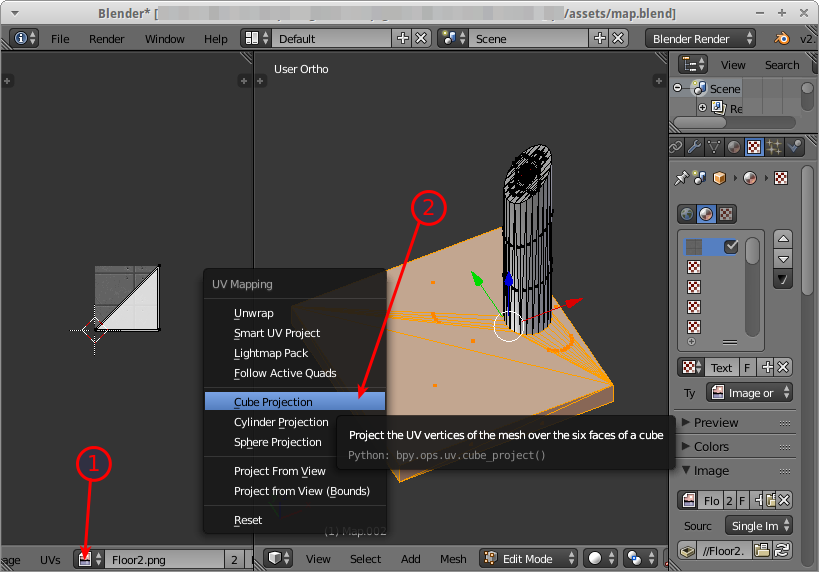
\includegraphics[scale=0.4]{blender_step10.png}
\step The mesh is now UV-mapped. You can see the result by selecting Texture in the Viewport Shading menu (1). In the image editor (2) are showing up the UV mapping of the select faces.\\
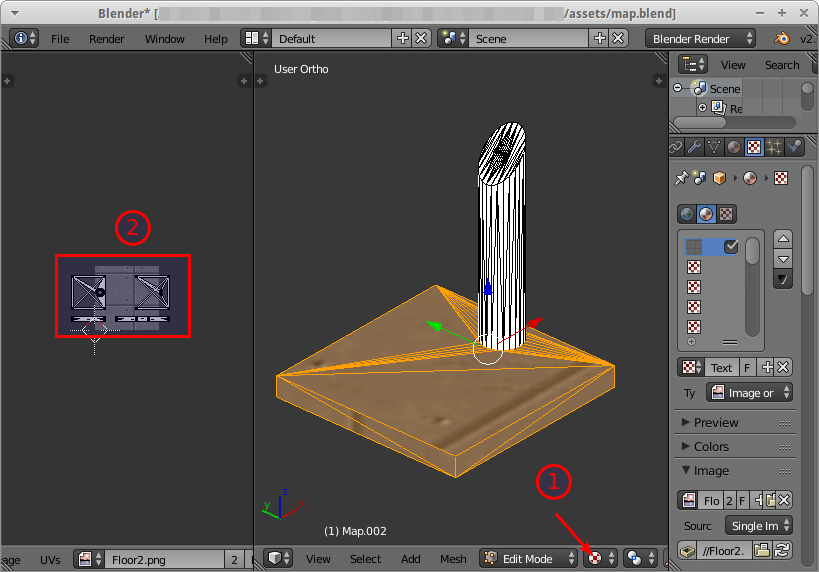
\includegraphics[scale=0.4]{blender_step11.png}
\begin{hint}
The Cube projection is especially useful here because it calculate an UV mapping appropriate for walls and makea proper synchronisation between walls so it looks continuous.
\end{hint}
\step The UV map is too small. We want the texture to be smaller and to repeat itself. In the image editor, select all faces \textbf{[A]} and scale \textbf{[S]} until the texture is small enough. I scaled x5 for my elevator.\\
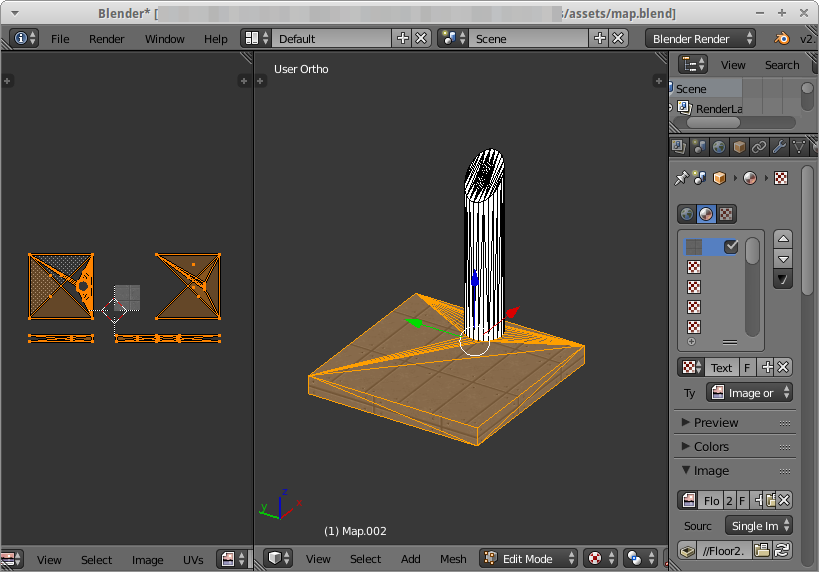
\includegraphics[scale=0.4]{blender_step12.png}
\begin{hint}
Sometimes the UV unwrap doesn't put the faces together, which results with a weird mapping when scaling the faces. But if you scale with a round number (by typing the number), it should always look fine. In the worst case, you can always manually correct the position of the faces, or use the "Project from View" unwrap option for the faces you want. With a bit of manual work, I fixed 2 faces who out of place.\\
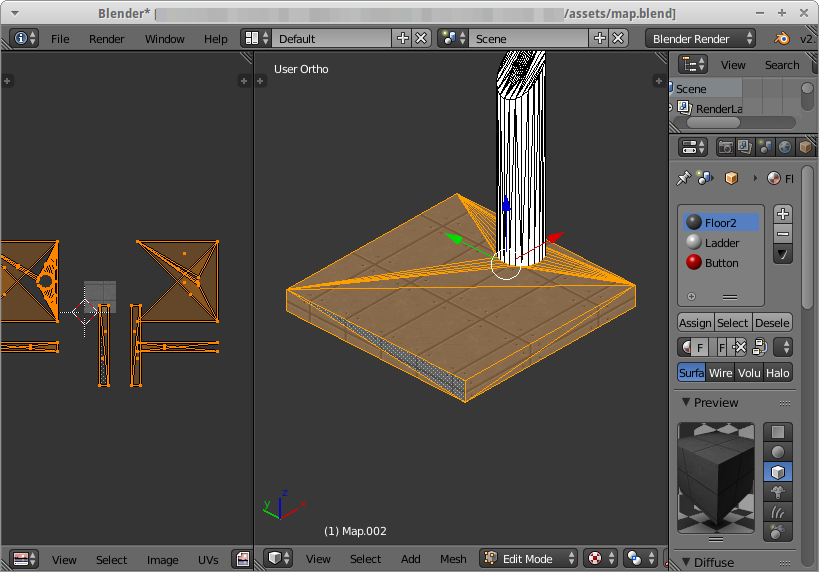
\includegraphics[scale=0.4]{blender_step13.png}
\end{hint}
\begin{hint}
The button and the tube are white even though they have a material. Don't panic, it's normal. The Texture View Shading shows only textures which are UV mapped, and materials with only a color are rendered in white. In the solid mode and the final rendering (if you add some lights), it looks fine.
\end{hint}
\step This mesh is now ready. Repeat the same process for all others meshes. You don't need to recreate a texture for the material slot you already assigned to a texture, because the material is shared between the meshes.
\step After that, your map should look a bit like this:\\
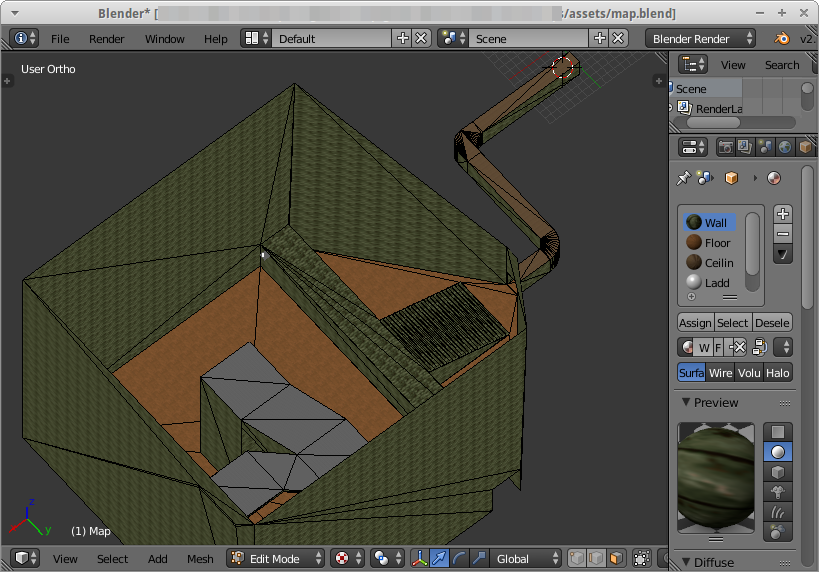
\includegraphics[scale=0.4]{blender_step14.png}
Once all meshes are UV mapped and all materials have a texture, this section is done and only remains the lights and the door.
\subsection{Lights}
Adding light is very simple, but in the same it can be a whole profession on itself just to get the proper lighting. But here we'll only see the simple version. 
\step Set the 3d cursor to where you want to add a light.
\step Add a point light with \textbf{[Shift-A]} and select Lamp / Point.
\step Change the Viewport Shading to Material so you can see the result.\\
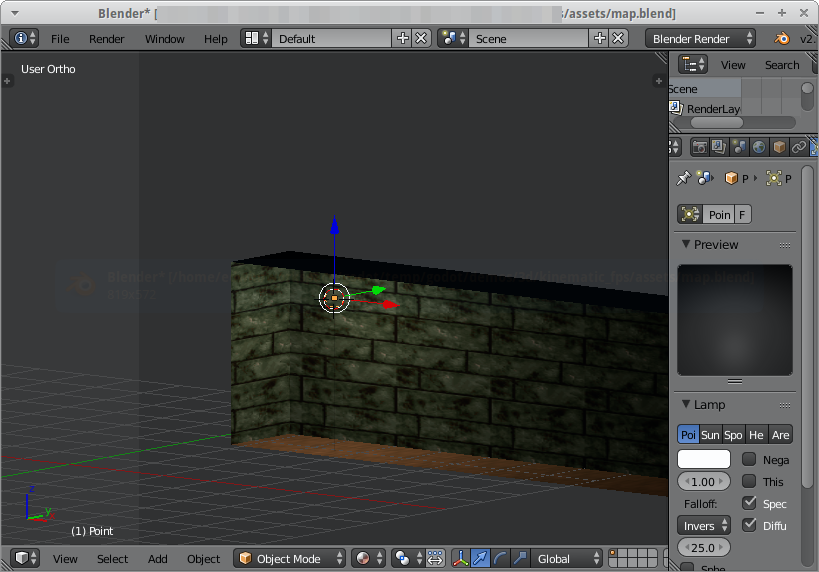
\includegraphics[scale=0.4]{blender_step15.png}
\step Change the Energy of the lamp and the color to your content.
\begin{hint}
If walls and floors seem to shine like plastic, reduce the specular intensity of the material.
\end{hint}
\step Repeat as much as needed.\\
\\
You have now a map with lights. Something like this:\\
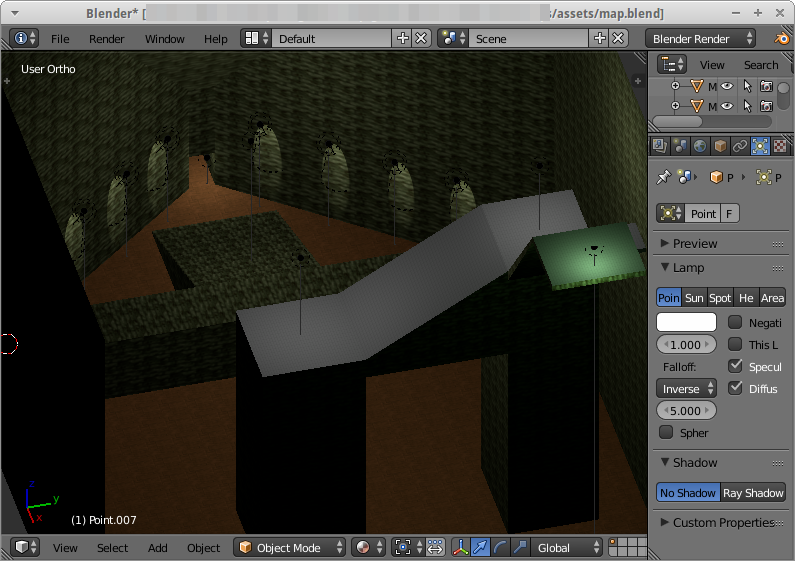
\includegraphics[scale=0.45]{blender_step16.png}
Now we're almost done with the assets.
\subsection{Doors}
Since we're at it, let's make a door. Just a simple one, like in the old game Doom\cite{doom}, which goes up when we activate it.
\step Put the 3d cursor to where you want the door and add a cube.\\
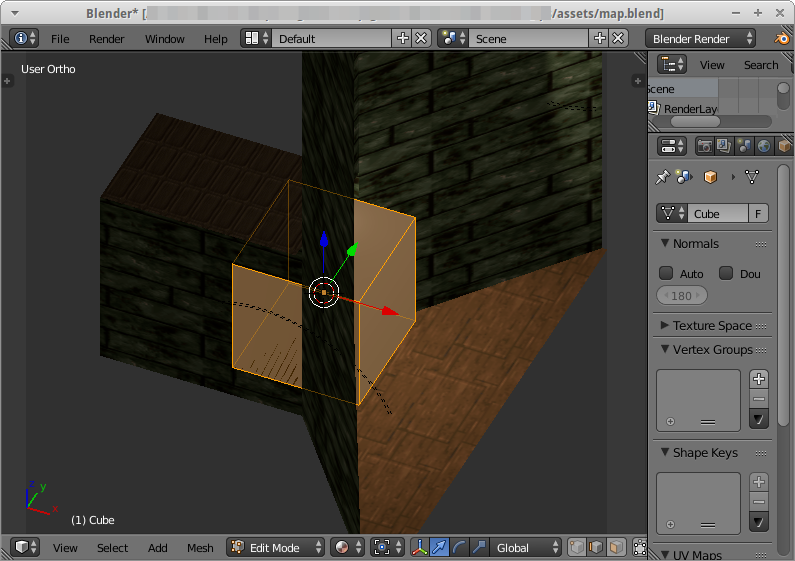
\includegraphics[scale=0.45]{blender_step17.png}
\step Go in edit mode and resize it to a vertical rectangle that covers the hallway.\\
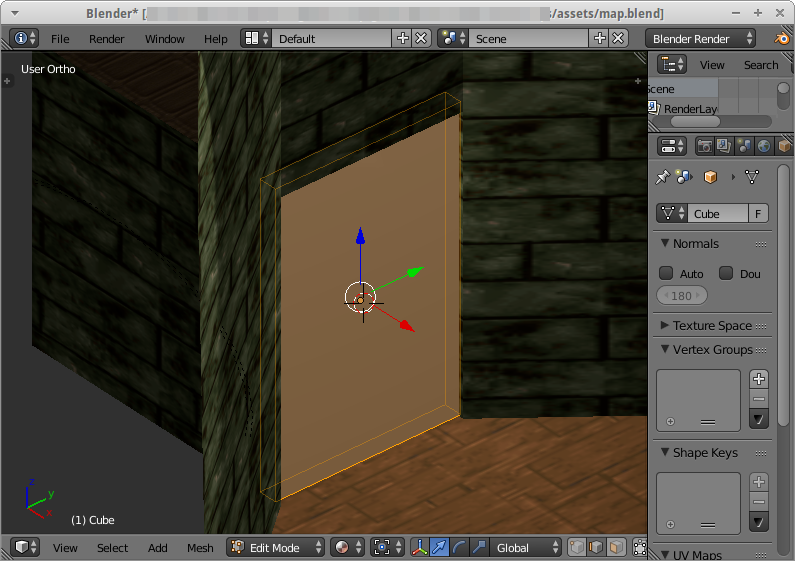
\includegraphics[scale=0.45]{blender_step18.png}
\step Give it a material and a color (or a texture, if you want).\\
\\
That's all.
\subsection{Names}
Before exporting the map to Godot, we must give a proper name to each mesh we created. Lights don't need a special name.
\step Select the main map object and rename it "Map-col".\\
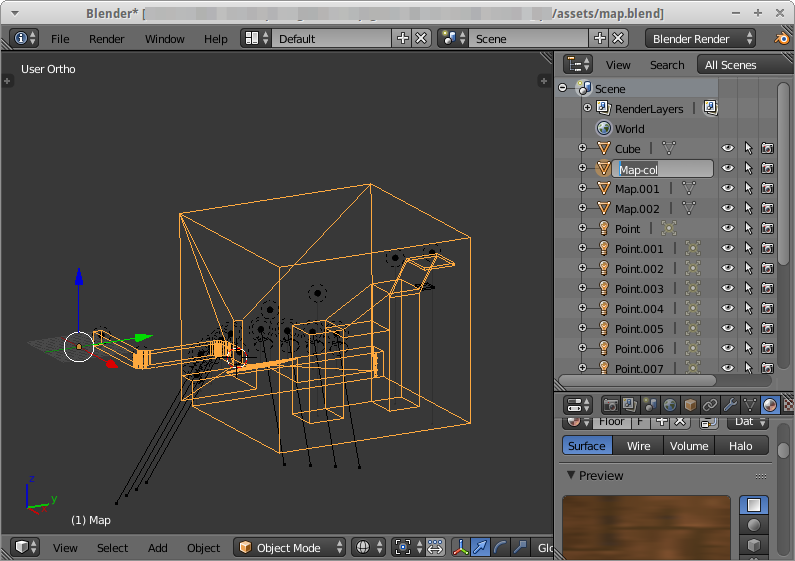
\includegraphics[scale=0.45]{blender_step19.png}
\begin{warning}
You must add the "-col" at the end of the name. The importer of Godot will understand that it is collidable, and it will automatically create a rigidbody node for the mesh.\\
You can check the wiki of Godot to know more about the others available options.
\end{warning}
\step Select the elevator meshes and rename them "Elevator1-col" and "Elevator2-col".
\step And finally rename the door as "Door-col".
\begin{hint}
You are free to choose whatever name you want. It is only important to keep the options like "-col" at the end as a suffix. Those suffixes won't appear in the name of the node in Godot. You can also combine options by adding them like this "My\_object-col-option1-option2-option3" (the name in Godot will be \textit{My\_object}).
\end{hint}
\subsection{Export to Collada}
Now the map is finally ready to be exported.
\step Save! If you didn't save your file until now, it is the time to do it \textbf{[Ctrl-S]}.
\step Enable the Collada exporter distributed with Godot if it's still not enabled.\\
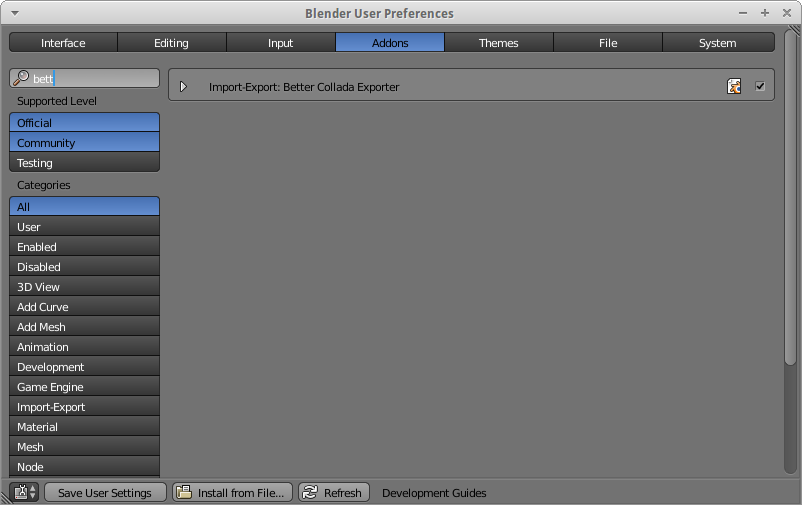
\includegraphics[scale=0.45]{blender_step20.png}
\step Open the menu File / Export / Better Collada (.dae)\\
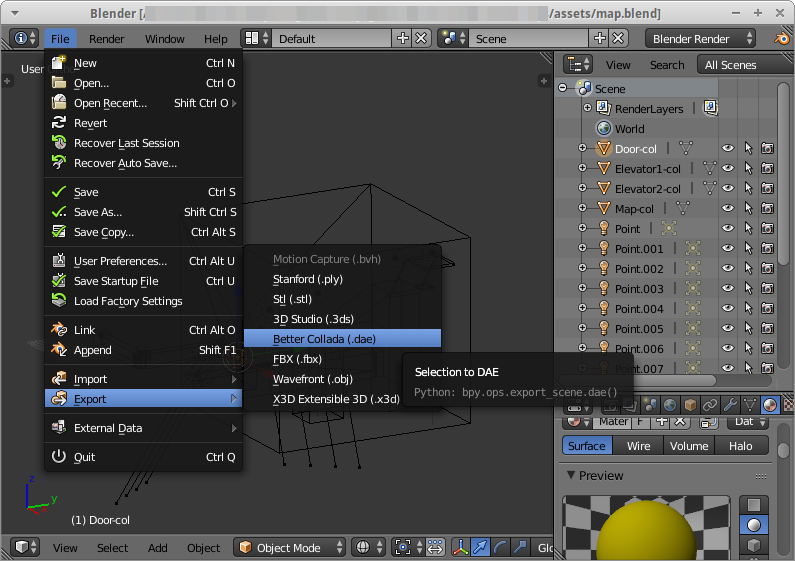
\includegraphics[scale=0.45]{blender_step21.png}
\step Set the following options:\\
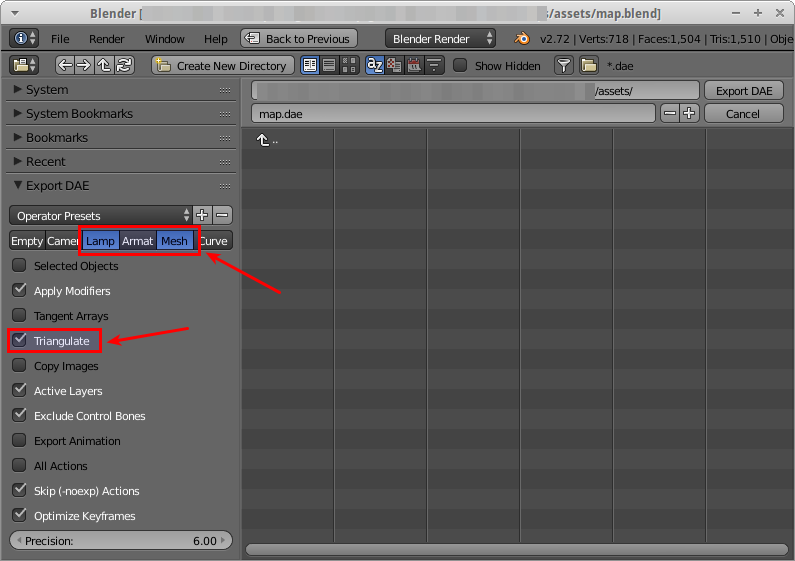
\includegraphics[scale=0.45]{blender_step22.png}
\step And then click the "Export DAE" button.
\step You can now close Blender.
\step You should have a .dae file in the "assets" folder. Copy this file in the "game\_assets" folder.\\
\\
That's it! Now you have a map, with elevators and a door. There's a button too, but it will be defined in Godot. Next, we'll import the scene in Godot and start with the main dish : physics!\\
\begin{hint}
You can find my .dae file and the texture in the "source/game\_assets" folder of my project in Github. And you can find the blender file in the "assets" folder, if you want.
\end{hint}
\section{Import the map in Godot}

\step Open the project in Godot.
\step In menu, Import / 3D scene.
\step Select as source scene the .dae file in the "game\_assets" folder.
\step Select "res://game\_assets" as target path
\step Disable Import Animations
\step Click on "Import \& Open"
\step You should now see the map\\
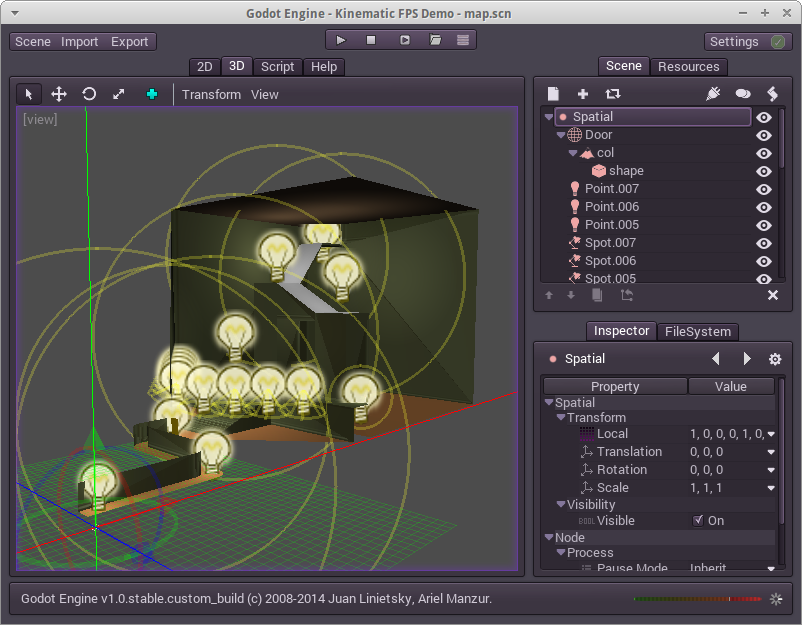
\includegraphics[scale=0.45]{godot_step1.png} 
\step Disable the default light in menu View, and ajust the lightning.\\
\\
You have maybe noticed that the textures seem off. At best only a part of the texture shows up.\\
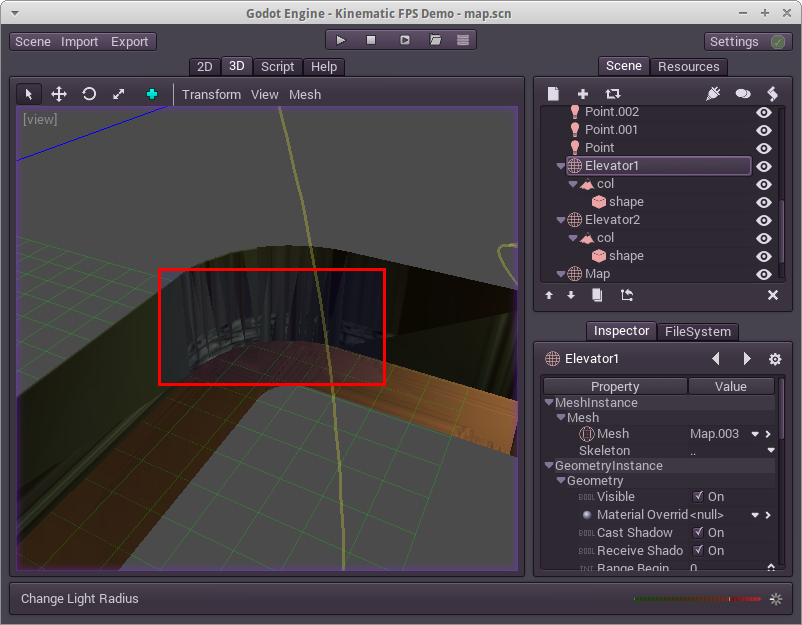
\includegraphics[scale=0.45]{godot_step2.png} 
That's because the texture is not repeated. We'll fix that.
\step Go in menu Import / 2D Texture.
\step As source, select all textures at once in the "game\_assets" folder.\\
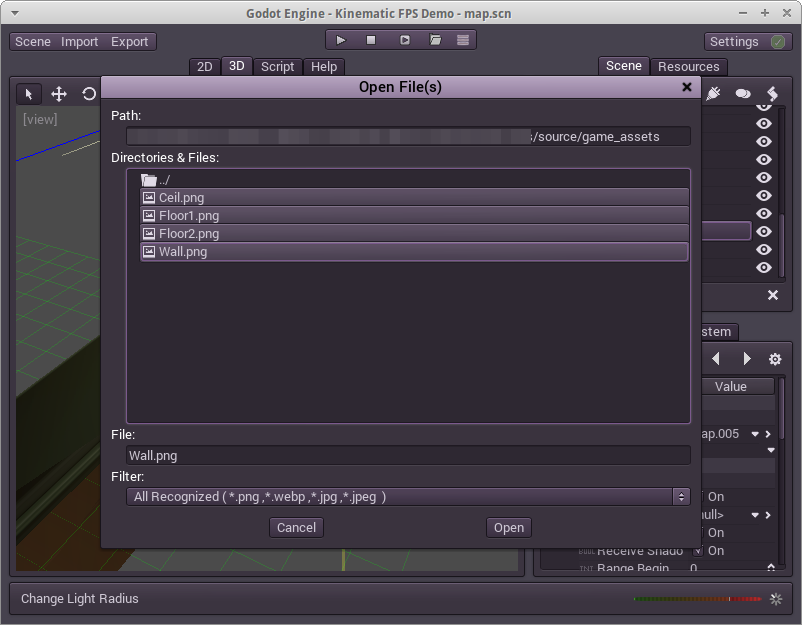
\includegraphics[scale=0.45]{godot_step3.png} 
\step Select "res://game\_assets" as target and check the repeat option.\\
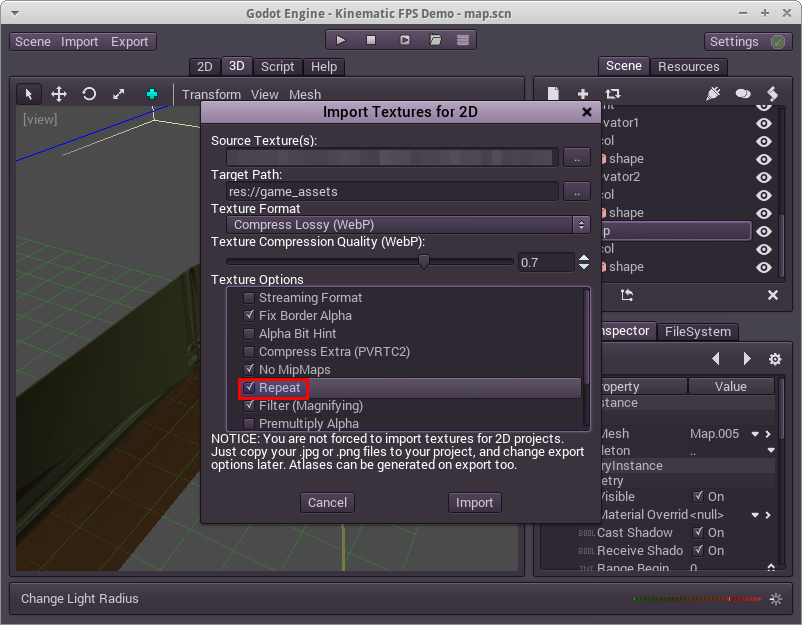
\includegraphics[scale=0.45]{godot_step4.png} 
\step Import.
\step Select the node of the map (1) and open its mesh property (2).\\
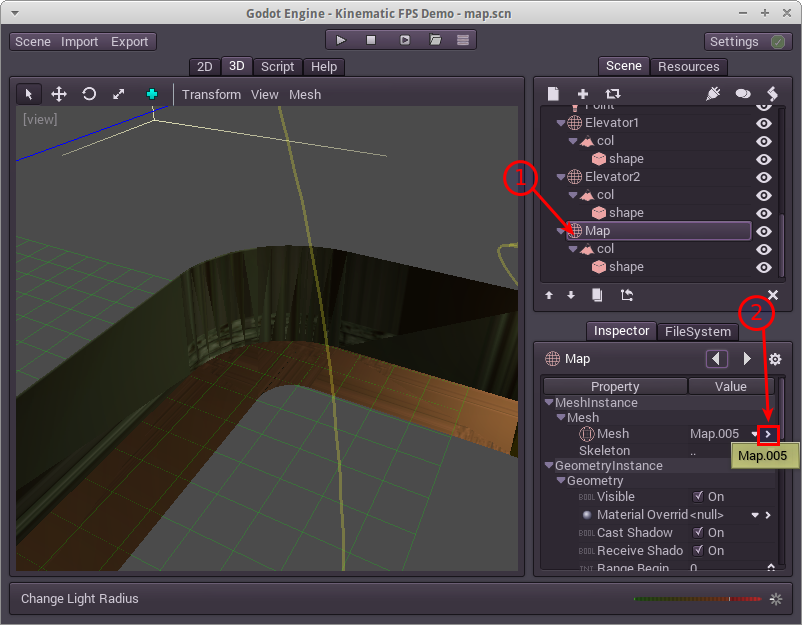
\includegraphics[scale=0.45]{godot_step5.png} 
\step You'll find multiple surfaces, which are the equivalent of materials in blender. Select the material of the first surface with a texture and open its details.\\
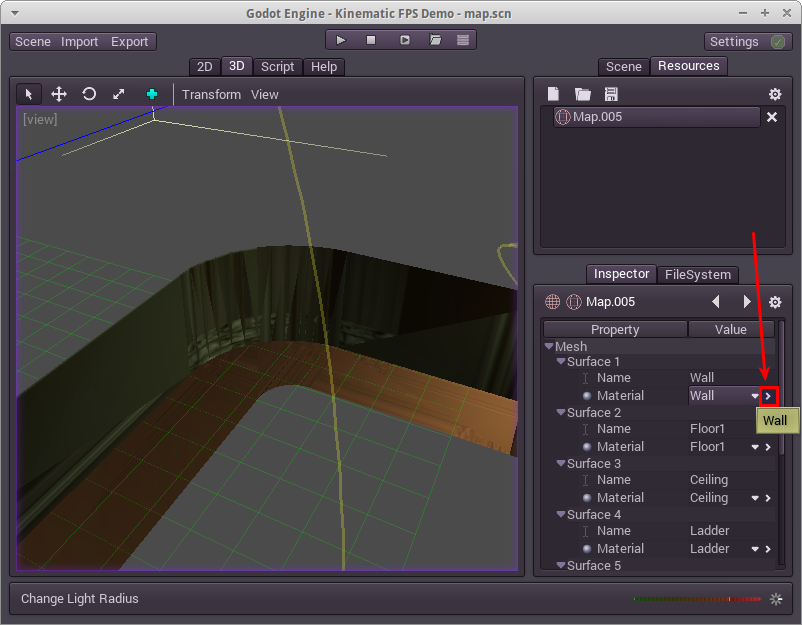
\includegraphics[scale=0.45]{godot_step6.png} 
\begin{hint}
During the import, the name of the material you gave in blender shows up here.
\end{hint}
\step You can see here all the options of the material. Go to the option Textures / Diffuse (1) and click on "Load" (2).\\
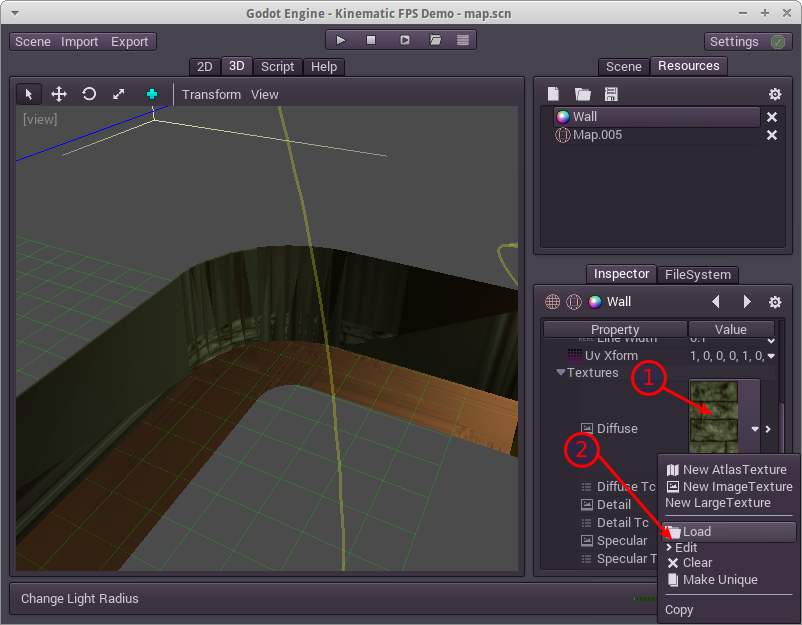
\includegraphics[scale=0.45]{godot_step7.png} 
\step Then choose the appropriate file with a .tex extension.\\
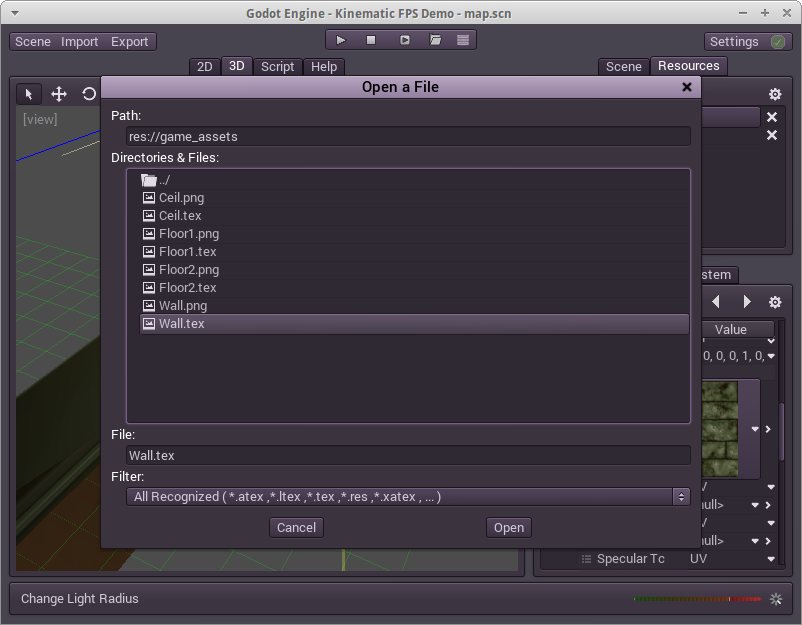
\includegraphics[scale=0.45]{godot_step8.png} 
\step The texture is now properly repeated.\\
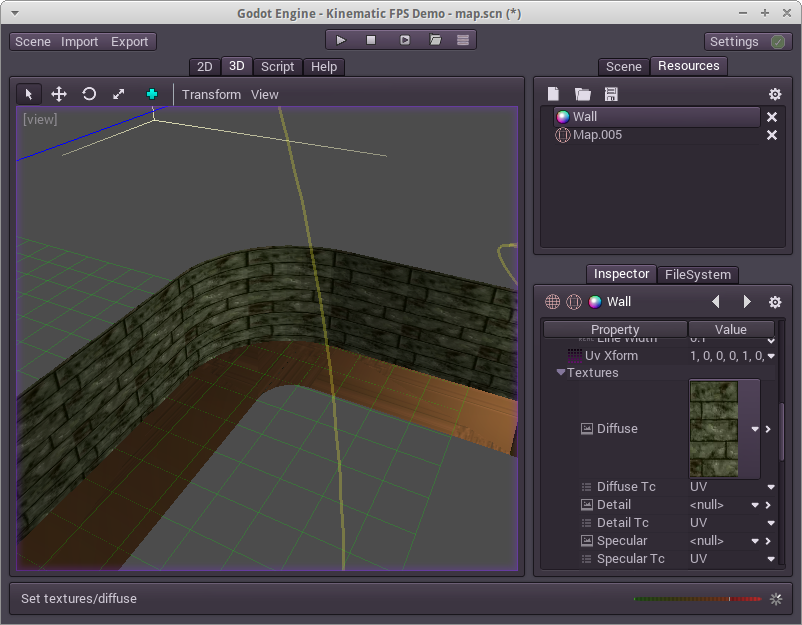
\includegraphics[scale=0.45]{godot_step9.png} 
\step Repeat the steps for each material of the scene.
\begin{hint}
No need to do it for materials without texture.
\end{hint}
At the end, you have a properly textured map.\\
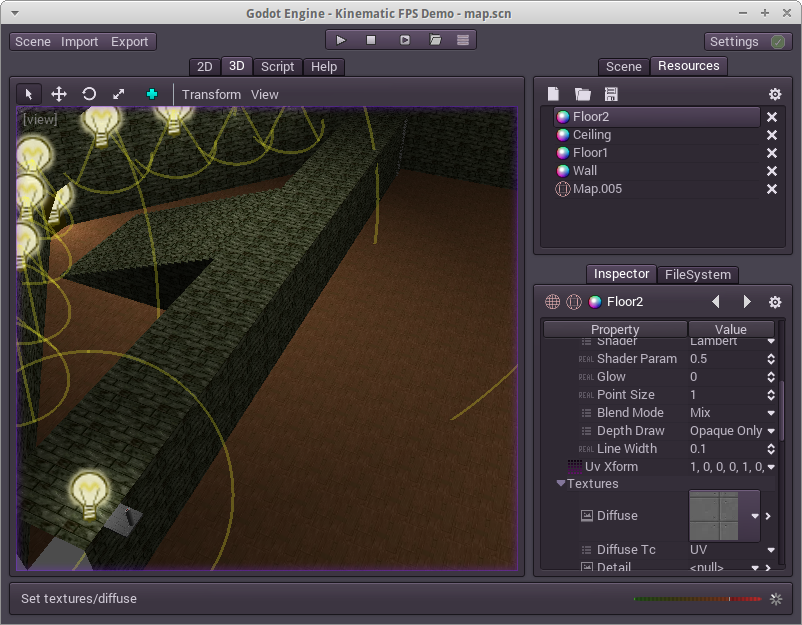
\includegraphics[scale=0.45]{godot_step10.png} 
\section{Main Scene}
Now that we have imported everything, let's create the main scene. It's better to modify as little as possible the imported scene because everything would be lost if you have to import it again.
\step Create a new scene in the menu Scene / New Scene.
\step Add a \textit{Spatial} node and name it \textit{World},
\step With the \textit{World} node selected, add an instance of a scene (1) and select the imported scene (2).\\
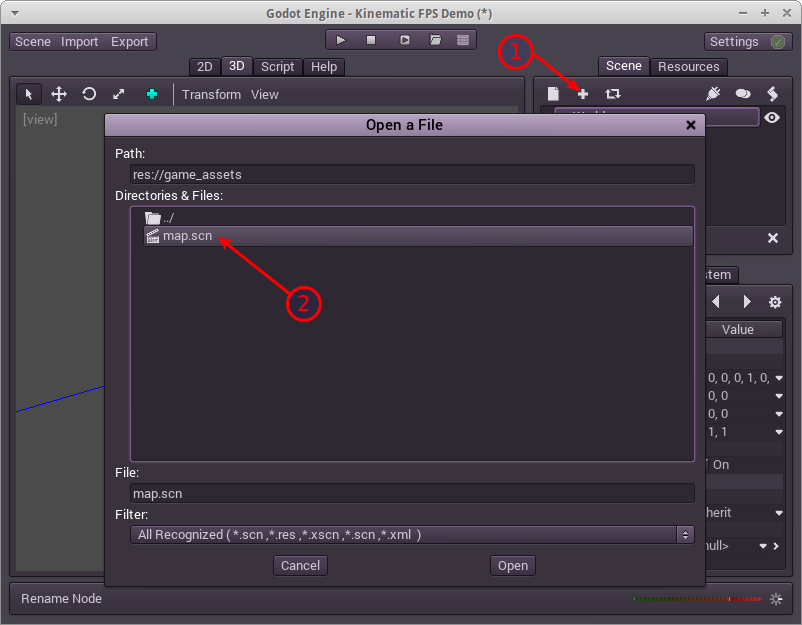
\includegraphics[scale=0.45]{godot_step11.png} 
\step The map is now showing up. Move it a bit vertically, for instance to y=1.
\begin{hint}
It's a small fix to a strange bug that happens when the player is at position y=0. It makes the player vibrate endlessly. Later, if you see such problem, elevate the map even more.
\end{hint}
\step Save the scene to "res://main.scn".
\step While we're at it, go in the project Settings and set the main\_scene to "res://main.scn".\\
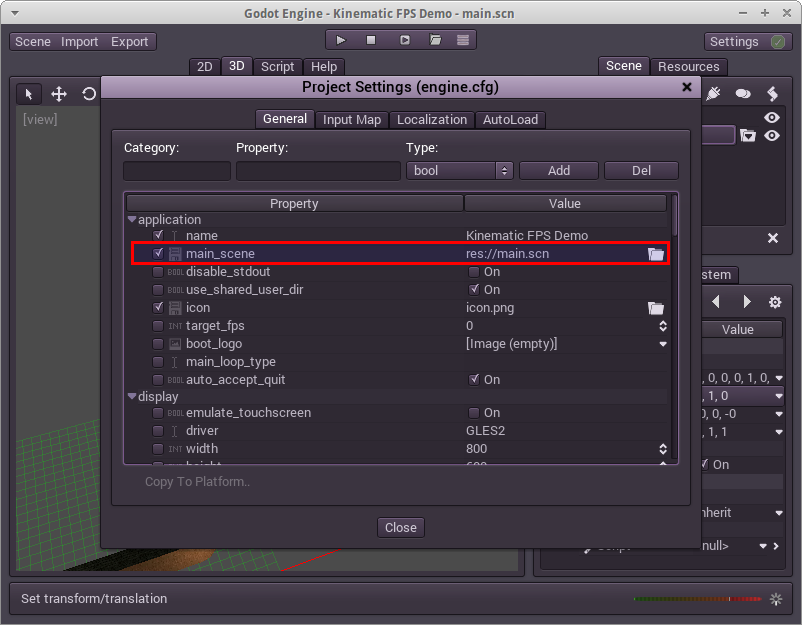
\includegraphics[scale=0.45]{godot_step12.png} \\
\\
Now we have a map and a main scene. We can finally work on the player.
\section{Player}

\subsection{Theory of kinematic objects}
Before we start, a bit of explanation.

\paragraph{Physics engine} Godot contains a physics engine that provides tools to detect collisions and calculate paths to slide along the colliding objects. It doesn't provide however a ready to use solution for a FPS character that can walk, jump and climb stairs. And that's what we're going to implement in GDScript.

\paragraph{Rigid body and kinematic body}
In Godot, a rigid body is an object that is managed completely by the physics engine. We can only manipulate it by giving force impulses to move it or set its position. But eventually it's moved by the physics engine and the result is hard to predict. The kinematic body is like a rigid body except that we have to make it move ourselves with a script. We must take care of its velocity, collision detection, gravity and everything. However we can use functions from the physics engine. And the most important one is \textit{move(...)}, which makes the body move to a specific direction, but only if it doesn't collide with something else. With this, we are certain that our object would never intersect with another object. It requires more work to use a kinematic body rather than a rigid body because we must take care of everything, but we have a complete control of our object.

\paragraph{Skeleton of a kinematic body} Technically a body can have any shape. In our tutorial, our character is a human. It doesn't need to be complex and a mere basic geometric shape is enough. In fact a mere box would be enough is most cases. If we take for instance a 2D platform game like Mario Bros (see fig. \ref{fig:mario_collision_shape}), the character collides with the ground and enemies as if it was just a rectangle (in yellow). You can also notice that in such game the rectangle never rotate or get transformed. Only its position change. In similar 3D games, it's the same concept, except that we use a box instead of a 2D rectangle. 

\paragraph{Collision and sliding} The physics engine calculates automatically the traject of the box by giving it a velocity. And if it encounters a wall, it will try to slide along the wall. At least, as much as possible. Because it the character tries to run directly against a wall, he won't slide at all. But if the velocity of the character goes a bit along the wall, the calculated velocity to slide  will be perpendicular to the wall. As shown in figure \ref{fig:collision_sliding}, the object at position $P$ moves with an initial velocity $V$ and collides at position $P_1$. A sliding velocity $S$ will be calculated and the object will move to its final position $P_2$.

\begin{figure}[h]
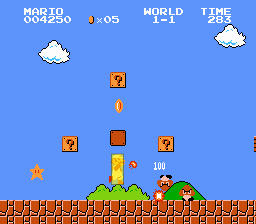
\includegraphics[scale=1]{NES_Super_Mario_Bros.png} 
\caption{Mario Bros on NES}
\label{fig:mario_collision_shape}
\end{figure}

\begin{figure}[h]
\centering
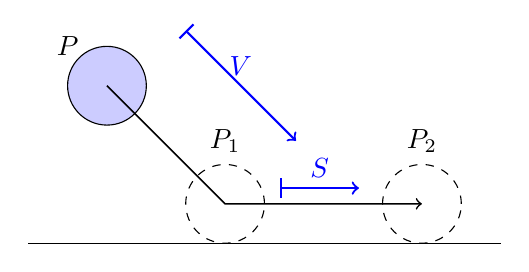
\begin{tikzpicture}
	\draw[fill=blue!20] (1,2) circle (5mm);
	\draw[dashed] (2.5,0.5) circle (5mm) ;
	\draw[dashed] (5,0.5) circle (5mm);
	\draw (0,0) -- (6,0);
	\draw[|->,thick,blue] (2,2.7) -- node[above] {$V$} ++(1.4,-1.4);
    \draw[|->,thick,blue] (3.2,0.7) -- node[above] {$S$} ++(1,0);
	\draw[->,semithick] (1,2) -- (2.5,0.5) -- (5,0.5);
	\draw (0.5,2.5) node {$P$};
	\draw (2.5,1.3) node {$P_1$};
	\draw (5,1.3) node {$P_2$};
\end{tikzpicture}
\caption{Collision and sliding}
\label{fig:collision_sliding}
\end{figure}

\paragraph{Problematic of the staircase}
With the sliding, a mere box is enough in most cases. Even with a slope, the box would be able to properly slide against it. However there is one case were the box doesn't suffice. Stairs. We humans can climb stairs thanks to our legs, but a box that slide against the floor would be stuck . The problem is that a stair is a wall but with a small height. However the physics engine do only detect there is a collision and it calculates the sliding velocity as if it was a wall. We must use another shape, which is the capsule. This shape has the particularity that its bottom is round (like an half sphere). When it collides against a stair, due to its round shape, the sliding velocity calculated will be different from sliding velocity of the rectangle shape, because the stair would be seen as a slope instead of a wall. As in figure \ref{fig:stair_problematic_1}, the sliding velocity of the box would be completely vertical. But because of the gravity, it would not move at all. However the sliding velocity of the capsule is like a slope, because it's the tangent of the half circle at the collision point. And as long as the slope is not too steep, the character would be able to climb it. No special scripting is needed. That's why the capsule shape is one popular way to solve this problem.

\begin{figure}[h]
\centering
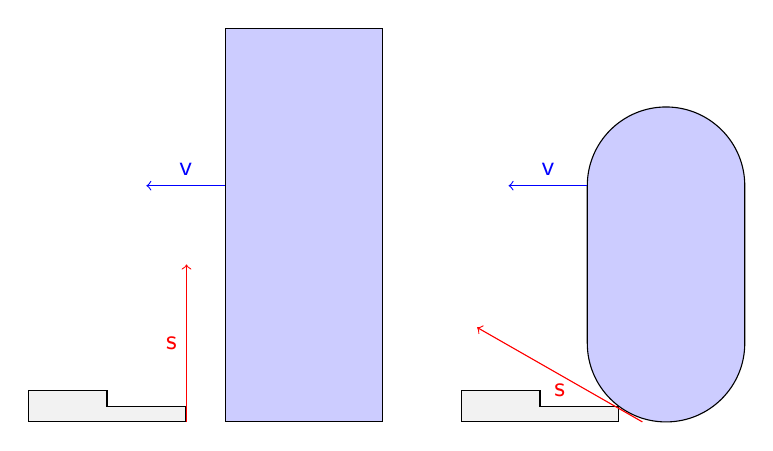
\begin{tikzpicture}
	\draw[fill=lightgray!20] (0,0) -- (0,0.4) -- (1,0.4) -- (1,0.2) -- (2,0.2) -- (2,0) -- (0,0);
	\draw[fill=blue!20] (2.5,0) rectangle (4.5,5);
	\draw[->,draw=blue] (2.5,3) -- node[above] {\color{blue}v} (1.5,3);
	\draw[->,draw=red] (2.01,0) -- node[left] {\color{red}s} (2.01,2);
	\draw[shift={(5.5,0)},fill=lightgray!20] (0,0) -- (0,0.4) -- (1,0.4) -- (1,0.2) -- (2,0.2) -- (2,0) -- (0,0);
	\draw[shift={(8.1,0)},fill=blue!20] (-1,1) arc (180:360:1) -- (1,3) arc (0:180:1) -- (-1,1);
	\draw[->,shift={(8.1,0)},draw=red] (-0.3,0) -- node [below] {\color{red}s} (-2.4,1.2);
	\draw[->,shift={(8.1,0)},draw=blue] (-1,3) -- node[above] {\color{blue}v} (-2,3);	
\end{tikzpicture}
\caption{Problematic of the staircase}
\label{fig:stair_problematic_1}
\end{figure}

\paragraph{Legs} But one constraint of this way is that the curve of the capsule must be very wide compared to the height of the stair. Practically it would be like the character could only climb up stairs of 1 cm high. Or the capsule must be very wide, meaning that our character is very fat. In both case, it's not very usable. Here comes the concept of leg. As in figure \ref{fig:kinematic_skeleton_1}, the capsule is elevated and a ray is stuck below. The ray is the representation of the human leg. When we think about it, the reason why the character can't climb too high stairs is that the tangent of the collision point is too steep, and that's because the collision point on the curve of the capsule is too high. By elevating the capsule, the collision point will be lower on the curve. And we use a ray for the leg because we need something to keep the capsule elevated but we don't want the leg to collide with the stair. The ray shape is special in the way that it has a width=0. It collides only on its length, here vertically.

\begin{figure}[h]
\centering
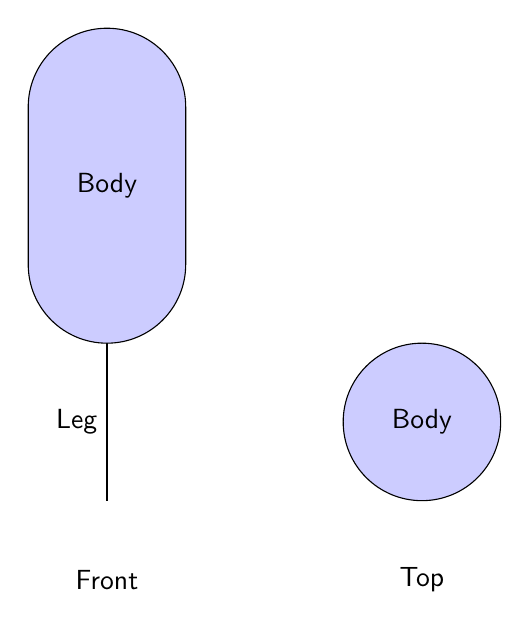
\begin{tikzpicture}
	\draw (0,0) -- node[left] {Leg} (0,2);
	\draw[fill=blue!20] (-1,3) arc (180:360:1cm) -- (1,5) arc (0:180:1cm) -- (-1,3);
	\node at (0,4) {Body};
	\draw[fill=blue!20] (4,1) circle (1cm) node {Body};
	\node at (0,-1) {Front};
	\node at (4,-1) {Top};
\end{tikzpicture}
\caption{Skeleton of the kinematic body, version 1}
\label{fig:kinematic_skeleton_1}
\end{figure}

\subsection{Fly mode}
\label{subsec:fly_mode}
\paragraph{Skeleton}
We will now implement a first version of this kinematic character. It is the most simplest one, the fly mode. This implementation, as its name say, doesn't have gravity. It can just move in space and collide with objects, like a ship in space. \\
\\
Let's start with the skeleton:
\step Create a new scene.
\step Add a \textit{KinematicBody} node and rename it \textit{actor}.
\step Save the scene as "actor.res" in the folder "res://".
\step Select the \textit{actor} node and add a \textit{CollisionShape} node, named as \textit{body}.
\step Select the \textit{body} node and in its Shape property create a new CapsuleShape.\\
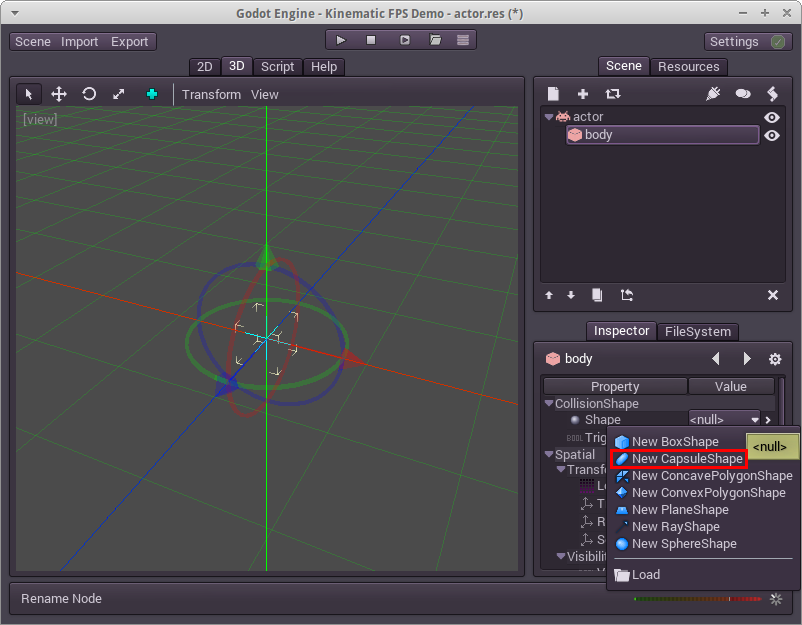
\includegraphics[scale=0.45]{godot_step13.png} 
\step Set its Translation to value [0,1.4,0] and its Rotation to [90,0,0].
\step Go in the detail of the property Shape.\\
\includegraphics[scale=0.45]{godot_step14.png} 
\step Set its Radius to 0.6 and its Height to 0.8
\step Select the \textit{body} node again.
\step Add another \textit{CollisionShape} node and rename it \textit{leg}.
\step For its shape, create a new RayShape.
\step Set its Translation to [0,0,1]
\step Go it the Shape detail and set value 0.4 for the Length property.
\step Select the \textit{actor} node and create a new \textit{Spatial} node. Rename it \textit{yaw}.
\step With the \textit{yaw} node selected, create a new \textit{Camera} node. Rename it \textit{camera}.
\step Set the Translation of \textit{camera} to [0,1.7,0], and check the option Current.\\
\\

Maybe you're wondering why I added a camera in an empty spatial node. The reason is that we want to keep the collision shapes as static, without rotation. Like in the old Mario game, the character itself doesn't rotate. This simplifies a lot the calculations since a lot of variables are now constants, thanks to this arbitrary rule to not rotate.\\
The only nodes that rotates are the yaw, only for horizontal rotation, and the camera for vertical rotation. Why not both in one node, you ask? Again, it's to simplify the maths in the script to come. One big difference between 2D math and 3D math is that rotations act differently depending on which axis of rotation is used. By separating the camera rotation in two rotations, it is easier to understand which axis of rotation we must use.

\paragraph{Set up the main scene}
Since we have the node of the player, even thought it does nothing, we can test it already.
\step Open the "main.scn" scene
\step Select the \textit{World} node
\step Instance the \textit{actor} node we just created and rename it \textit{player}
\step Move the node somewhere in the map. That will be its original position.\\
\\
You can now give it a try and start the scene \textbf{[F5]}. You should normally see the map from where you put your \textit{player} node.

\paragraph{Keys}
Before we continue, it is a good idea to configure now the keys we're going to use in this tutorial.
\step Open the project settings and go in Input map tab.
\step Add the following actions : move\_forward, move\_backward, move\_left, move\_right, jump, use
\step For each action, add the key you want. Personally I use the WASD configuration for movement, with space and E for jump and use.
\step Close the window.

\paragraph{Scripting}
\step Open the "actor.res" scene.
\step Select \textit{actor} node and click on the "Create the node script" button\\
\includegraphics[scale=0.45]{godot_step15.png} 
\step Click "Create" button
\step Replace the content of the script with this code:
\begin{pythoncode}
  extends KinematicBody
  
  func _input(ie):
    pass
  
  func _fixed_process(delta):
    pass
  
  func _ready():
    set_fixed_process(true)
    set_process_input(true)
\end{pythoncode}
\begin{hint}
The process input function is called whenever a button is pressed or the cursor is moved. In our case, we'll capture the mouse movement here.
\end{hint}

Now that we have the most basic structure of the code, we're going to implement the capture of the mouse movements.
\step At the beginning of the script, after the \textit{extends KinematicBody} line, add those variables:
\begin{pythoncode}
  var view_sensitivity = 0.3
  var yaw = 0
  var pitch = 0
\end{pythoncode}
\step In the \_input(ie) function, replace the content with this code:
\begin{pythoncode}
  if ie.type == InputEvent.MOUSE_MOTION:
    yaw = fmod(yaw - ie.relative_x * view_sensitivity, 360)
    pitch = max(min(pitch - ie.relative_y * view_sensitivity, 90), -90)
    get_node("yaw").set_rotation(Vector3(0, deg2rad(yaw), 0))
    get_node("yaw/camera").set_rotation(Vector3(deg2rad(pitch), 0, 0))
\end{pythoncode}
\begin{hint}
The variables \textit{yaw} and \textit{pitch} are the rotations of the camera. As explained before, we apply the \textit{yaw} rotation to the spatial parent of the camera instead of the camera, as we do for the pitch. Also, since we capture the delta of the mouse movements, we must check that the yaw angle doesn't go too high or negative. Therefore we apply a modulo to this value. For the pitch, we put a limit instead so the camera's orientation is always with the up on the top of the screen. Since the actor's body never rotate vertically, the camera must have the same up orientation as the body.
\end{hint}
\step Append at the end of the script this code:
\begin{pythoncode}
  func _enter_tree():
    Input.set_mouse_mode(Input.MOUSE_MODE_CAPTURED)

  func _exit_tree():
    Input.set_mouse_mode(Input.MOUSE_MODE_VISIBLE)
\end{pythoncode}
\begin{hint}
This makes the game capture completely the mouse. You won't even see cursor. But this is required to let the camera be able to move easily in every direction. It has however the problem that you can only quit the game with a hotkey (\textbf{[Alt-F4]} or a key you program yourself to quit the game). It is particularly annoying when Godot suddenly stops because of a script error, because there's no other way than try to kill the process to get the mouse back (and you have to do it without mouse!). Be sure to know the useful hotkeys of your OS before you try a Godot code that captures the mouse. For Ubuntu, \textbf{[Super-T]} opens a terminal, and you can find the process with ps and kill it. In Windows, \textbf{[Ctrl-Shift-Esc]} opens the task manager. But it's safer to disable the \textit{set\_mouse\_mode(...)} code whenever you are not sure.
\end{hint}
If you try to run the game now, you should be able to move the camera with the mouse in every direction. Take note that no matter how much you rotate, the ceiling is always above the screen and the floor is always below (except if you look at it directly).

\paragraph{Move the actor}
We can now focus on make the actor move when we press a key.\\
The algorithm is described in figure \ref{fig:fly_mode_algo}. Take note that in the fly mode, velocity is at every frame set to zero. Thus there's no inertia.\\
Also, it is not shown in the diagram, but because the slide function of Godot is not perfect at the time I'm writing the tutorial, the actual implementation tries a couple of times to slide the actor until it doesn't slide anymore. This trick is only needed in the fly mode.

\begin{figure}[H]
\centering
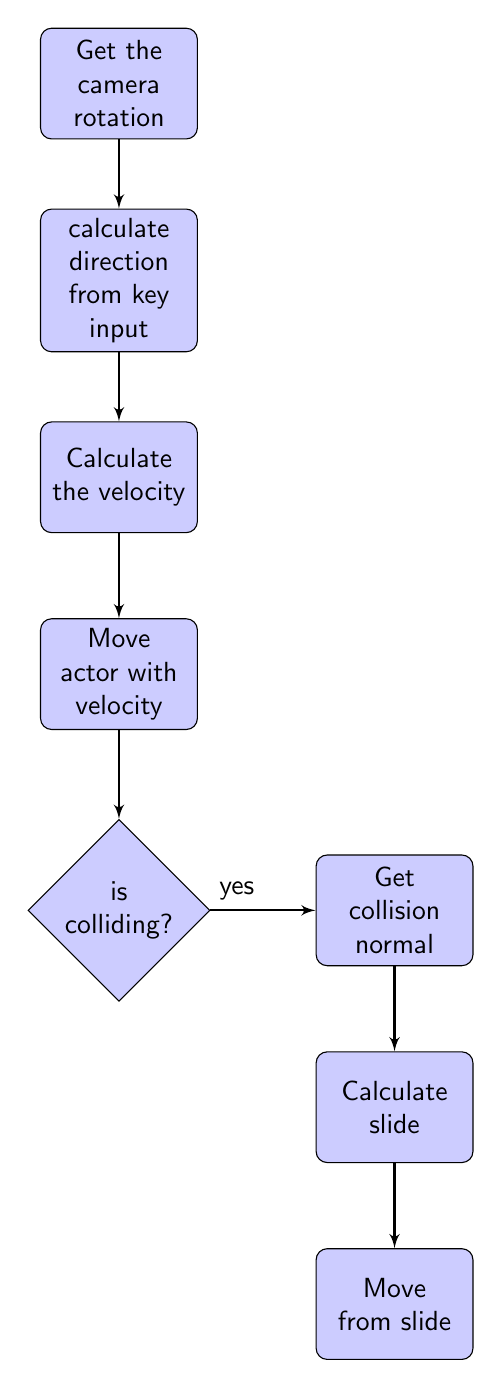
\begin{tikzpicture}[node distance = 2.5cm, auto]
   \node [block] (camera_rotation) {Get the camera rotation};
   \node [block,below of=camera_rotation] (input_key) {calculate direction from key input};
   \node [block,below of=input_key] (calc_velocity) {Calculate the velocity};   
   \node [block,below of=calc_velocity] (move) {Move actor with velocity};   
   \node [decision,below of=move] (if_collide) {is colliding?};   
   \node [block,right of=if_collide,node distance = 3.5cm] (collision_normal) {Get collision normal};      
   \node [block,below of=collision_normal] (slide) {Calculate slide};   
   \node [block,below of=slide] (move_slide) {Move from slide};   
   \path [line] (camera_rotation) -- (input_key);
   \path [line] (input_key) -- (calc_velocity);
   \path [line] (calc_velocity) -- (move);
   \path [line] (move) -- (if_collide);
   \path [line] (if_collide) -- node [near start] {yes} (collision_normal);   
   \path [line] (collision_normal) -- (slide);
   \path [line] (slide) -- (move_slide);
\end{tikzpicture}
\caption{Algorithm of the fly mode}
\label{fig:fly_mode_algo}
\end{figure}

\step Add those variables and constants with the others variables:
\begin{pythoncode}
  var velocity=Vector3()
  
  const FLY_SPEED=100
  const FLY_ACCEL=4
\end{pythoncode}
\step Append at the end of the script:
\begin{pythoncode}
  func _fly(delta):
    # read the rotation of the camera
    var aim = get_node("yaw/camera").get_global_transform().basis
    # calculate the direction where the player want to move
    var direction = Vector3()
    if Input.is_action_pressed("move_forward"):
      direction -= aim[2]
    if Input.is_action_pressed("move_backward"):
      direction += aim[2]
    if Input.is_action_pressed("move_left"):
      direction -= aim[0]
    if Input.is_action_pressed("move_right"):
      direction += aim[0]

    direction = direction.normalized()
        
    # calculate the target where the player want to move
    var target=direction*FLY_SPEED

    # calculate the velocity to move the player toward the target
    velocity=Vector3().linear_interpolate(target,FLY_ACCEL*delta)

    # move the node
    var motion=velocity*delta
    motion=move(motion)

    # slide until it doesn't need to slide anymore, 
    #or after n times
    var original_vel=velocity
    var attempts=4 # number of attempts to slide the node

    while(attempts and is_colliding()):
      var n=get_collision_normal()
      motion=n.slide(motion)
      velocity=n.slide(velocity)
      # check that the resulting velocity is not opposite to 
      # the original velocity, which would mean moving backward.
      if(original_vel.dot(velocity)>0):
          motion=move(motion)
          if (motion.length()<0.001):
            break
      attempts-=1     
\end{pythoncode}
\begin{hint}
You might have noticed there is a strange \textit{Vector3().linear\_interpolate} function call. In fact, the \textit{Vector3()} is normally the old velocity from last frame. But since we don't want to keep the velocity in fly mode, I replaced it with a new empty vector, meaning no velocity.
\end{hint}
\begin{hint}
Another interesting line to understand is the \textit{get\_node("yaw/camera").get\_global\_transform().basis}.\\
More detail in the annexe chapter \ref{subsec:camera_aiming} about camera aiming.
\end{hint}
\step And finally replace the content of function \textit{\_fixed\_process} with:
\begin{pythoncode}
  _fly(delta)
\end{pythoncode}

If you run now the game, you should be able to move in your map.\\
\begin{hint}
You can find the complete script and scene for the actor at this point in the project's folder "tutorial/fly\_mode".
\end{hint}

\subsection{Walk mode}
\step Before we go further, make a copy of the \textit{\_fly} function and rename the copy \textit{\_walk}. 
\begin{warning}
Don't change directly the \textit{\_fly}function, we'll need it later.
\end{warning}
\step change the content of \textit{\_fixed\_process} to :
\begin{pythoncode}
  _walk(delta)
\end{pythoncode}

\subsubsection{Velocity}
\step In the fields/variables section, add the following code:
\begin{pythoncode}
  const WALK_MAX_SPEED = 15
  const ACCEL= 2
  const DEACCEL= 4 
  
  var is_moving=false
\end{pythoncode}
\step At the beginning of the \textit{\_walk} function, just before \textit{direction = direction.normalized()}, add:
\begin{pythoncode}
  #reset the flag for actora's movement state
  is_moving=(direction.length()>0)
\end{pythoncode}
\step Replace this line:
\begin{pythoncode}
  var target=direction*FLY_SPEED
\end{pythoncode}
with
\begin{pythoncode}
  var target=direction*WALK_MAX_SPEED
  # if the character is moving, he must accelerate. 
  # Otherwise he deccelerates.
  var accel=DEACCEL
  if is_moving:
    accel=ACCEL
\end{pythoncode}
\step Replace this line:
\begin{pythoncode}
  # calculate the velocity to move the player toward the target
  velocity=Vector3().linear_interpolate(target,FLY_ACCEL*delta)
\end{pythoncode}
with
\begin{pythoncode}
  # calculate velocity's change
  var hvel=velocity
  hvel.y=0
	
  # calculate the velocity to move toward the target, 
  # but only on the horizontal plane XZ
  hvel=hvel.linear_interpolate(target,accel*delta)
  velocity.x=hvel.x
  velocity.z=hvel.z
\end{pythoncode}

Give it a try and run the game. ...Hey! We can't climb up in the air anymore! It's like we're stuck on an imaginary floor.\\
\\
That's right. The changes we did just now added inertia to our velocity (you've maybe noticed that when you stop walking, you slow down first) but only on the horizontal plane. We nullified the Y value in the direction we try to go. That's because when we walk, we're stuck to the ground thanks to gravity. We can then consider that we have only the ability to move on a 2D plan, jumping being an exception. It looks weird now, but once we implement gravity it will make more sense.
\begin{hint}
We added at the same time the variable \textit{is\_moving}. It will have multiple uses later, but now it helps to know if the actor must accelerate or decelerate. Because in video game physics, friction can be simplified by considering that there's friction only when something is not moving by itself. And when it wants to move, it accelerates before it reaches the maximum speed.
\end{hint}
\begin{hint}
Did you also noticed that the speed changed? And on top of that it seems there is a maximum speed we can't go beyond. That's thanks to the \textit{linear\_interpolate} function. This function calculate a vector based on another vector and a length. If the length is bigger than the reference vector's length, it will be capped to the reference vector's length.
\end{hint}
\subsubsection{Gravity}
\step Add this code to the fields/variables section:
\begin{pythoncode}
  const GRAVITY=-9.8*3
\end{pythoncode}
\begin{hint}
Gravity is multiplied 3 times because it gives a better feeling. I'm not sure why, but it's probably related to a unit conversion problem (9.81 is the gravity acceleration constant in $m*s^{2}$, but there's no meter unit in Godot). You can change it to your content.
\end{hint}
\step After \textit{direction = direction.normalized()}, add:
\begin{pythoncode}
  # add gravity
  velocity.y+=delta*GRAVITY
\end{pythoncode}

If you test it now, you'll see yourself falling to the ground. And if you go on a slope, you slide down to the bottom, no matter how steep the slope is. However you can see that depending on how steep the slope is, you have more or less difficulty to climb it. And check for the stairs. If you made a staircase that have low stairs, you'll be able to climb up the staircase, but not easily. That's thanks to ours capsule shape.
\paragraph{Congratulation!} You made your very first FPS character. It's from far not perfect, but it walks on the ground and it falls. It can even climb slopes and stairs (somehow).\\
\\
Now we're going to fix all those problems.\\
\begin{hint}
You can find the complete script and scene for the actor at this point in the project's folder "tutorial/basic\_gravity".
\end{hint}

\subsubsection{Jump}
Jumping is a simple matter of giving a vertical impulse.
\step Add in the field section:
\begin{pythoncode}
  const JUMP_SPEED = 3*3
\end{pythoncode}
\step Add at the end of the function:
\begin{pythoncode}
  if Input.is_action_pressed("jump"):
    velocity.y=JUMP_SPEED
\end{pythoncode}
If you try it, you see that you can now jump vertically. But as long as you press the jump key, you jump. Even in the middle of the air. We need to add a condition to allow to jump only when we're on the ground. But this comes in the next chapter.
\subsubsection{Ground-clamping}
\label{subsec:ground_clamping}
If you played a bit with the current state of the game, you might have noticed a couple of problems:
\begin{itemize}
\item You can't stay on a slope, no matter how low it is. It's like you're standing on ice.
\item Jumping should be allowed only when you're on floor.
\item When you walk on a slope from the top, you're jumping first before you slide down.
\end{itemize}
All issues point to the need to detect when the character touches the floor. Not only but also the last issue is a bit more complicated. In figure \ref{fig:basic_gravity_slope}, you see the actor on a slope. If the actor has a velocity, it's a horizontal velocity. It means that when the actor moves, he will lose foot for an instant, and then he'll fall due to gravity (in red). If the velocity is small, it is unnoticeable, especially now that the actor can't even stand still on the slope. But if he goes faster, he'll be constantly falling, as if he jumps down. What we want instead is that the actor follows the ground (in blue). But for that, we need to make the actor to stick to the ground. This is what we call ground clamping.

\begin{figure}[H]
\centering
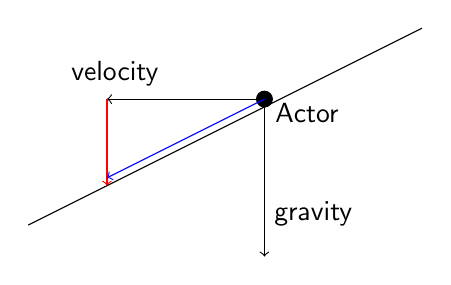
\begin{tikzpicture}
\draw [domain=-3:2] plot(\x,{-0.1+\x*1/2});
\draw [fill=black] (0,0) circle (0.1);
\draw [->] (0,0) -- (-2,0);
\draw [->] (0,0) -- (0,-2);
\draw [->,color=red] (-2,0) -- (-2,-1.1);
\draw [->,color=blue] (0,0) -- (-2,-1);
\draw[color=black] (0.54,-0.18) node {Actor};
\draw[color=black] (-1.9,0.32) node {velocity};
\draw[color=black] (0.62,-1.46) node {gravity};
\end{tikzpicture}
\caption{Problem of sliding down a slope from a side view}
\label{fig:basic_gravity_slope}
\end{figure}

\paragraph{Raycast} The approach to solve those problems is to add a \textit{raycast} below the player like in figure \ref{fig:kinematic_skeleton_2}, and if a collision is detected, teleport the player to the collision point.

\begin{figure}[H]
\centering
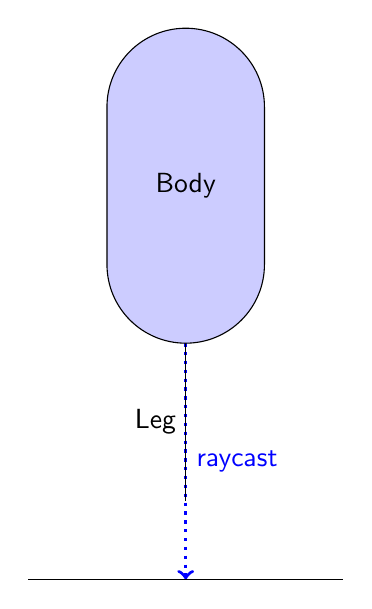
\begin{tikzpicture}
	\draw [->,color=blue,dotted,very thick](0,2) -- node[right] {raycast} (0,-1);
	\draw (0,0) -- node[left] {Leg} (0,2);
	\draw[fill=blue!20] (-1,3) arc (180:360:1cm) -- (1,5) arc (0:180:1cm) -- (-1,3);
	\node at (0,4) {Body};
	\draw (-2,-1) -- (2,-1);
\end{tikzpicture}
\caption{Skeleton of the kinematic body, version 2}
\label{fig:kinematic_skeleton_2}
\end{figure}

The length of the ray is quite important, because on a slope it will be the tolerance margin to consider that the actor is still on the ground, as shown in figure \ref{fig:raycast_slope}. If the ray is too short and the velocity is too high, the actor would be in the air the moment it reaches a slope, then fall. \\
But on the other side the ray must not be too long, because it would be like the actor is always touching the ground.

\begin{figure}[H]
\centering
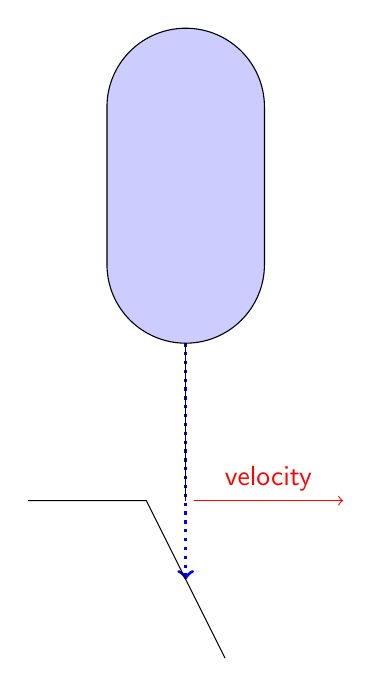
\begin{tikzpicture}
	\draw [->,color=blue,dotted,very thick](0,2) -- (0,-1);
	\draw (0,0) -- (0,2);
	\draw[fill=blue!20] (-1,3) arc (180:360:1cm) -- (1,5) arc (0:180:1cm) -- (-1,3);
	\draw (-2,0) -- (-0.5,0) -- (0.5,-2);
	\draw [->,color=red](0.1,0) -- node[above] {velocity} (2,0);
\end{tikzpicture}
\caption{Margin of the raycast on a slope}
\label{fig:raycast_slope}
\end{figure}

\paragraph{Implementation}
\step In the scene tree of the actor, select the \textit{actor} node.
\step Add a \textit{RayCast} node (don't confuse with \textit{RayCast2D}) and name it \textit{ray}.
\step Move it to \textit{Translation} [0,0.4,0], just at the intersection between \textit{body} and \textit{leg} nodes.
\step Check property \textit{Enabled}
\step Set the property \textit{Cast To} to [0,-0.8,0]\\
You should now have a scene structure like this:\\
\includegraphics[scale=0.45]{godot_step16.png} 
It's hard to see where the \textit{ray} node is, but it's in the red rectangle I've drawn.

\step In the script file, add in the fields section:
\begin{pythoncode}
  var on_floor=false
\end{pythoncode}
\step Add at the very beginning of the \textit{\_walk} function:
\begin{pythoncode}
  var ray = get_node("ray")
\end{pythoncode}
\step Replace the code:
\begin{pythoncode}
  direction = direction.normalized()
\end{pythoncode}
with:
\begin{pythoncode}
  direction.y=0
  direction = direction.normalized()
	
  # clamp to ground if not jumping. Check only the first time a 
  # collision is detected (landing from a fall)
  var is_ray_colliding=ray.is_colliding()
\end{pythoncode}
\begin{hint}
For convenience we nullify right here the Y of the direction. We are sure now that the actor moves only horizontally.
\end{hint}
\step Right after that, add the following code:
\begin{pythoncode}
  if !on_floor and is_ray_colliding:
    set_translation(ray.get_collision_point())
    on_floor=true
  elif on_floor and not is_ray_colliding:
    # check that flag on_floor still reflects the state of the ray.
    on_floor=false
\end{pythoncode}		
\begin{hint}
Here we did 2 things. Not only we clamp to the ground the actor when he detected the collision, which we know it's the ground since it's right bellow, but we also configured a flag(field) \textit{on\_floor} to whether if the actor is on the floor or in air. You might have noticed that we teleport the actor only if there is a change between the collision state of the ray and the flag. By not constantly teleport the actor to the ground, not only we avoid useless code that would only slow down (a little) the game, but it avoids also possible bugs of the player moving vertically for no reason (for instance in an elevator).
\end{hint}
\step Replace the code:
\begin{pythoncode}
  # add gravity
  velocity.y+=delta*GRAVITY
\end{pythoncode}
with:
\begin{pythoncode}
  if on_floor:
    pass
  else:
    # apply gravity if falling
    velocity.y+=delta*GRAVITY
\end{pythoncode}
\begin{hint}
Gravity is now applied only when the actor is in the air. He doesn't slide anymore when he's on a slope. But it doesn't consider the angle of the slope for the moment.
\end{hint}
\step We can simplify the motion part. Replace:
\begin{pythoncode}
  var attempts=4 # number of attempts to slide the node
	
  while(attempts and is_colliding()):
    var n=get_collision_normal()
    motion=n.slide(motion)
    velocity=n.slide(velocity)
    # check that the resulting velocity is not opposite to the 
    # original velocity, which would mean moving backward.
    if(original_vel.dot(velocity)>0):
      motion=move(motion)
      if (motion.length()<0.001):
        break
    attempts-=1
\end{pythoncode}
with:
\begin{pythoncode}
  if(motion.length()>0 and is_colliding()):
    var n=get_collision_normal()
    motion=n.slide(motion)
    velocity=n.slide(velocity)
    # check that the resulting velocity is not opposite to the 
    # original velocity, which would mean moving backward.
    if(original_vel.dot(velocity)>0):
      motion=move(motion)
\end{pythoncode}
\begin{hint}
It does the same thing as before, but because our way to calculate the velocity changed, I noticed with practice that multiple move attempts are not needed anymore. I've then only removed everything that became useless and that would only slow the game down.\\
And I added a condition. If the actor doesn't move (\textit{motion.length==0}), no need to do all this extra calculation.
\end{hint}

\step Let's finish with the jump. Replace:
\begin{pythoncode}
  if Input.is_action_pressed("jump"):
	  velocity.y=JUMP_SPEED
\end{pythoncode}
with:
\begin{pythoncode}
  if on_floor:
    if Input.is_action_pressed("jump"):
      velocity.y=JUMP_SPEED
\end{pythoncode}

Now give it a try. We can't fly with the jump key anymore. And we can stand on a slope, though it's not perfect and we still slide slowly.\\
However new bugs appeared. When you climb a slope and stop, you're elevating in the air before you suddenly teleport to the ground. And when you going down the slope, you're first falling before you slide down. The reason it that the gravity is not applied all the time anymore and the vertical velocity .\\\\
It's definitely not perfect. But we'll fix all this.

\begin{hint}
You can find the complete script and scene for the actor at this point in the project's folder "tutorial/ground\_clamping".
\end{hint}

\subsubsection{Slopes}
\label{subsec:slopes}
In the previous section, what is missing is the part to manage the vertical velocity. When you move, the X and Z of the actor's velocity accelerate. And when you touch nothing, the X and Z of the actor's velocity decelerate. But in a slope, the Y changes too due to the \textit{slide} function. However, when you don't move anymore, the Y of the velocity doesn't decelerate and the actor starts to elevate until it reaches the point where the ray doesn't detect the ground anymore. And then the actor falls and the Y axis of its velocity is set to 0.\\
In figure \ref{fig:problem_climb_slope}, step 1. shows the actor moving with a velocity. \\
Step 2. show the actor when the player doesn't press a movement key; the X velocity is decelarated to 0 but the remaining Y velocity is still there. \\
Step 3. shows the actor in the air and its ray that doesn't touch the ground anymore. Gravity applies again and the actor starts to fall.

\begin{figure}[H]
\centering
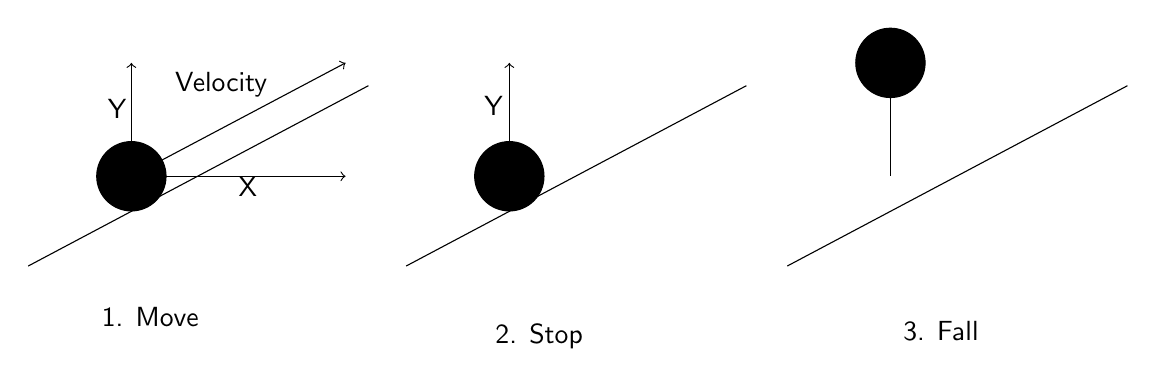
\begin{tikzpicture}
\draw [fill=black,fill opacity=1.0] (0,0.44) circle (0.44cm);
\draw [fill=black,fill opacity=1.0] (4.8,0.44) circle (0.44cm);
\draw [fill=black,fill opacity=1.0] (9.64,1.88) circle (0.44cm);
\draw [->] (0,0.44) -- (2.72,1.88);
\draw [->] (0,0.44) -- (0,1.88);
\draw [->] (0,0.44) -- (2.72,0.44);
\draw (-1.31,-0.7)-- (3.01,1.59);
\draw (3.49,-0.7)-- (7.81,1.59);
\draw [->] (4.8,0.44) -- (4.8,1.88);
\draw (8.33,-0.7)-- (12.65,1.59);
\draw (9.64,1.88)-- (9.64,0.44);
\draw (-0.5,-1.1) node[anchor=north west] {1. Move};
\draw (4.5,-1.32) node[anchor=north west] {2. Stop};
\draw (9.68,-1.28) node[anchor=north west] {3. Fall};
\draw[color=black] (1.14,1.6) node {Velocity};
\draw[color=black] (-0.18,1.3) node {Y};
\draw[color=black] (1.48,0.3) node {X};
\draw[color=black] (4.6,1.34) node {Y};
\end{tikzpicture}
\caption{Problem of Y velocity when climbing the slope}
\label{fig:problem_climb_slope}
\end{figure}

As well, when running down a slope, the actor starts by walking horizontally until the ray doesn't touch the ground anymore and then starts to fall and follow the slope because of the gravity. That's because as long as the actor's ray touches the ground and the flag \textit{on\_floor} is true, the actor thinks he's on the floor and doesn't need to apply gravity.\\
To fix that, we need to adapt the velocity to the floor. As you can see in figure \ref{fig:slope_projection}, the actor has a remaining velocity $vel_0$ from previous frame. The actor collides with the ground thanks to the raycast, and the normal of the ground at the collision point is known as $normal$. By projecting $vel_0$ to the ground, perpendicularly to $normal$, we can get a velocity $vel_1$ that impacts the Y value of the original velocity. And this will solve both issues explained before, since the Y value of velocity will be indirectly decelerated.

\begin{figure}[H]
\centering
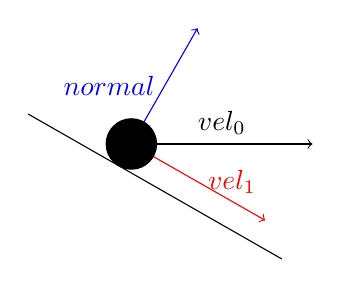
\begin{tikzpicture}
\draw [->,color=red] (0,0) -- node[right] {$vel_1$} (1.7,-0.97);
\draw [->] (0,0) -- node[above] {$vel_0$} (2.3,0);
\draw (-1.31,0.38)-- (1.91,-1.46);
\draw [->,color=blue] (0,0) -- node[left] {$normal$} (0.84,1.47);
\draw [fill=black,fill opacity=1.0] (0,0) circle (0.32cm);
\end{tikzpicture}
\caption{Project the velocity to the ground}
\label{fig:slope_projection}
\end{figure}

To do that, we use a scalar projection based on the normal of the ground. More explanations about scalar projection at chapter \ref{subsec:ortho_projection}.

\step In the script file, add in the fields section:
\begin{pythoncode}
  const MAX_SLOPE_ANGLE = 40
\end{pythoncode}
\step Replace the code:
\begin{pythoncode}
  if on_floor:
    pass
  else:
    # apply gravity if falling
    velocity.y+=delta*GRAVITY
\end{pythoncode}
with:
\begin{pythoncode}
  if on_floor:
    # if on floor move along the floor. To do so, we calculate the 
    # velocity perpendicular to the normal of the floor.
    var n=ray.get_collision_normal()
    velocity=velocity-velocity.dot(n)*n
		
    # apply gravity if on a slope too steep
    if (rad2deg(acos(n.dot(Vector3(0,1,0))))> MAX_SLOPE_ANGLE):
      velocity.y+=delta*GRAVITY
  else:
    # apply gravity if falling
    velocity.y+=delta*GRAVITY
\end{pythoncode}

Give it a try.\\
\\
That's quite good! Now we're totally sticking to the ground. And we don't slide at all on the slope that's not too steep, as well as we can't climb the other slope that is too steep. In fact, we stick so well to the ground that we can't even jump anymore, nor climb stairs (or very hardly). That's because the jump impulse we give is transformed to be parallel to the ground, which this time shouldn't be the case. But we are in the right direction. We just need to implement a couple of tricks.

\begin{hint}
You can find the complete script and scene for the actor at this point in the project's folder "tutorial/slopes".
\end{hint}

\subsubsection{Jumping again}
Jumping is not possible anymore because the ground clamping works too well. One simple solution for that is to temporarily disable the ground clamping to give to the actor the time to jump.

\step In the script file, add in the fields section:
\begin{pythoncode}
  var jump_timeout=0
  
  const MAX_JUMP_TIMEOUT=0.2
\end{pythoncode}
\step At the beginning of the \textit{\_walk} function, add:
\begin{pythoncode}
  # process timers
  if jump_timeout>0:
    jump_timeout-=delta
\end{pythoncode}

\step Replace the code:
\begin{pythoncode}
    if !on_floor and is_ray_colliding:
\end{pythoncode}
with:
\begin{pythoncode}
    if !on_floor and jump_timeout<=0 and is_ray_colliding:
\end{pythoncode}

\step Replace the code:
\begin{pythoncode}
    if Input.is_action_pressed("jump"):
      velocity.y=JUMP_SPEED
\end{pythoncode}
with:
\begin{pythoncode}
    if Input.is_action_pressed("jump"):
      velocity.y=JUMP_SPEED
      jump_timeout=MAX_JUMP_TIMEOUT
      on_floor=false
\end{pythoncode}

Try it. We can now jump again. What's left are the stairs.

\begin{hint}
You can find the complete script and scene for the actor at this point in the project's folder "tutorial/jump\_again".
\end{hint}

\subsubsection{Stairs}
For the problem of the staircase we'll use another trick. We'll use another raycast to detect stairs. If a stair is detected and if it's at the direction the actor is trying to move, we'll make the actor automatically jump. The concept is as described in figure \ref{fig:step_raycast} by putting a raycast in front of the actor. This step raycast must not collide with the ground and thus must be placed hight than the \textit{leg}. This raycast will be only used when the player moves and it will be positioned always where the actor is going, meaning the velocity's direction.

\begin{figure}[H]
\centering
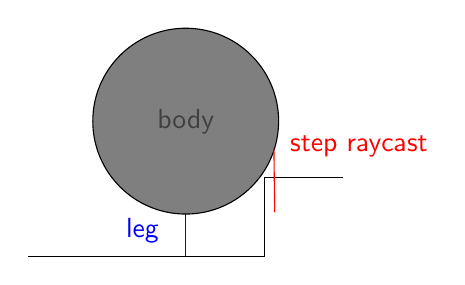
\begin{tikzpicture}
\draw [fill=black,fill opacity=0.5] (0,1.72) circle (1.18cm) node {body};
\draw (0,0)-- (1,0);
\draw (1,0)-- (1,1);
\draw (1,1)-- (2,1);
\draw [color=blue] (0,0.54)-- (0,0);
\draw [color=red] (1.12,1.38)-- (1.13,0.56);
\draw (0,0)-- (-2,0);
\draw[color=blue] (-0.55,0.33) node {leg};
\draw[color=red] (2.2,1.4) node {step raycast};
\end{tikzpicture}
\caption{Side view of the step raycast detecting a stair}
\label{fig:step_raycast}
\end{figure}
First we complete the player's skeleton:
\step In the scene tree, select the \textit{actor} node and add a \textit{RayCast} node. Call it \textit{stepRay}.
\step Mark it \textit{Enabled} and give it a \textit{Cast To} to [0,-0.5,0]
\step Move it to \textit{Translation} [0,0.75,-0.58], like this:\\
\includegraphics[scale=0.45]{godot_step17.png} 
Then we implement the script:
\step In the script file, add in the fields section:
\begin{pythoncode}
  const STAIR_RAYCAST_HEIGHT=0.75
  const STAIR_RAYCAST_DISTANCE=0.58
  const STAIR_JUMP_SPEED=5
  const STAIR_JUMP_TIMEOUT=0.2  
\end{pythoncode}
\step In function \textit{\_walk}, after the line:
\begin{pythoncode}
  var ray = get_node("ray")
\end{pythoncode}
add the line:
\begin{pythoncode}
  var step_ray=get_node("stepRay")
\end{pythoncode}
\step Replace the code:
\begin{pythoncode}
  if on_floor:
    # if on floor move along the floor. To do so, we calculate the 
    # velocity perpendicular to the normal of the floor.
    var n=ray.get_collision_normal()
    velocity=velocity-velocity.dot(n)*n
		
    # apply gravity if on a slope too steep
    if (rad2deg(acos(n.dot(Vector3(0,1,0))))> MAX_SLOPE_ANGLE):
      velocity.y+=delta*GRAVITY
  else:
    # apply gravity if falling
    velocity.y+=delta*GRAVITY
\end{pythoncode}
with:
\begin{pythoncode}
  if on_floor:
    # if on floor move along the floor. To do so, we calculate the 
    # velocity perpendicular to the normal of the floor.
    var n=ray.get_collision_normal()
    velocity=velocity-velocity.dot(n)*n
		
    # if the character is in front of a stair, and if the step is 
    # flat enough, jump to the step.
    if is_moving and step_ray.is_colliding():
      var step_normal=step_ray.get_collision_normal()
      if (rad2deg(acos(step_normal.dot(Vector3(0,1,0))))< MAX_SLOPE_ANGLE):
        velocity.y=STAIR_JUMP_SPEED
        jump_timeout=STAIR_JUMP_TIMEOUT		
		
    # apply gravity if on a slope too steep
    if (rad2deg(acos(n.dot(Vector3(0,1,0))))> MAX_SLOPE_ANGLE):
      velocity.y+=delta*GRAVITY
  else:
    # apply gravity if falling
    velocity.y+=delta*GRAVITY
\end{pythoncode}
\step And finally, add at the end of the function:
\begin{pythoncode}
  # update the position of the raycast for stairs to where the 
  # character is trying to go, so it will cast the ray at the next 
  # loop.
  if is_moving:
    var sensor_position=Vector3(direction.z,0,-direction.x)*STAIR_RAYCAST_DISTANCE
    sensor_position.y=STAIR_RAYCAST_HEIGHT
    step_ray.set_translation(sensor_position)
\end{pythoncode}
\begin{hint}
This last code calculates a position from the resulting velocity of this frame step, and then set the \textit{stepRay} at this position. Since the ray is a child of the \textit{actor}, its position is relative.
\end{hint}
Let's try it.\\\\
Much better! We can now climb stairs. It's not very fluid. If you compare with the old Doom\cite{doom} game, the player in Doom could climb stairs without losing velocity, where here the actor is more or less slowed down depending on the stairs height. But the way Doom was made is completely different from actual physics like the one Godot uses, and it wasn't exactly realistic anyway. For this tutorial, it will be more than enough.\\
\\
That's it. We finished the implementation of a kinematic FPS character. You could create a map and put this node in it, and you'll be able to visit this map.\\
However, the tutorial doesn't end here. Everything is fine, but only as long as the character doesn't interact with moving objects nor actionable objects (buttons, doors, ladders). The next chapters will cover those special aspects.

\begin{hint}
You can find the complete script and scene for the actor at this point in the project's folder "tutorial/climbing\_stairs".
\end{hint}


\section{Elevators}
We are now going to make things move in this map. The simplest ones are the elevators and moving platforms. Alas, they are also not the most intuitive (for the moment) to animate with our actor implementation.

\paragraph{Elevators} are imported as meshes that are part of the map but still are separate objects. Normally you should see in your scene in Godot that elevators were imported as separate nodes. 

\paragraph{Animation} In Godot, you can animate a node very easily thanks to a special node \textit{AnimationPlayer}. This allows you to change attributes, including \textit{Translation}, in a timeline that you define. The most obvious and easiest way to move an elevator from point A to point B is to set the \textit{Translation} property to both points at desired time. However if an object stands on this elevator, it won't move automatically with the elevator. For instance, if the player stands on a platform that moves horizontally, the platform would move while the player stand still. And eventually the player will fall of the platform. The problem is that no friction is applied to objects on top of the moving platform. Only when the elevator moves only vertically can objects follow the elevator because of the gravity. Otherwise they must be moving themselves with the elevator.

\paragraph{Linear velocity}
At the moment I'm writing this tutorial, I still didn't find a way to calculate the real velocity of an elevator when it's animated with an \textit{AnimationPlayer}. However, one of the demos I based my work on, called FPS Test \cite{FPSTest}, used the \textit{Angular Velocity} property of a \textit{RigidBody}. This property makes the object rotate on itself at specified speed, without using any \textit{AnimationPlayer}. Beside this property, there's the \textit{Linear Velocity} property which moves the object the same way as the \textit{Angular Velocity} rotates the object. If you set a non null vector to it, the body moves exactly at the speed of this vector. And since this vector can be accessed by others nodes, the trick when the player stands on the object is to read this vector and make the player move with the same velocity, on top of its own velocity but without changing it.\\
\\
The problem is that makes more complicated to configure the elevator. You can with the \textit{AnimationPlayer} change the \textit{Linear Velocity} at any time with the desired velocity, but you have to calculated the correct velocity to make the platform arrive on time at destination, not too late nor too soon. And most of the time you'll have to find with lot of tries the right velocity. Probably someone will find a more convenient solution soon.

\subsection{Preparation of the elevator node}
When the map was imported, the evelators, as well as all others meshes, were imported in 3 nodes like in figure \ref{fig:col_node_structure}.

\begin{figure}[H]
\centering
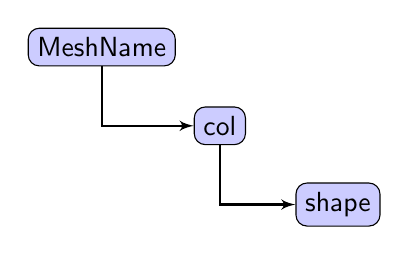
\begin{tikzpicture}[>=stealth',shorten >=1pt,auto, every node/.style={align=center}]
  \node[node] (mesh) {MeshName};
  \node[node,right of=mesh,below of=mesh,xshift=5mm] (col) {col};
  \node[node,right of=col,below of=col,xshift=5mm] (shape) {shape};

  \begin{scope}[every path/.style=line]
    \path (mesh) |- (col);
    \path (col) |- (shape);
  \end{scope}
  
\end{tikzpicture}
\caption{Elevator node structure}
\label{fig:col_node_structure}
\end{figure}

We want to swap the mesh and \textit{col} nodes, because the \textit{Linear Velocity} property is in \textit{col}. At the end, we want a structure like figure \ref{fig:corrected_col_node_structure}.
\begin{figure}[H]
\centering
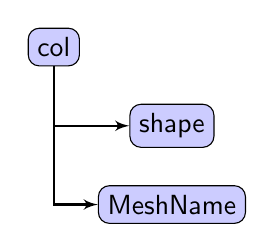
\begin{tikzpicture}[>=stealth',shorten >=1pt,auto, every node/.style={align=center,anchor=west}]
  \node[node] (col) {col};
  \node[node,right of=col,below of=col,xshift=5mm] (shape) {shape};
  \node[node,below of=shape] (mesh) {MeshName};

  \begin{scope}[every path/.style=line]
    \path (col) |- (mesh);
    \path (col) |- (shape);
  \end{scope}
  
\end{tikzpicture}
\caption{Corrected node structure}
\label{fig:corrected_col_node_structure}
\end{figure}

\step Open the map scene
\step Search for one elevator's node and select its \textit{col} node. Rename it a unique name related to the elevator's name, for instance \textit{col-elevator2} (because my mesh was named elevator2).
\step With the node still selected(1), reparent (2) it to the root node of the scene, usually name \textit{Spatial} by default.\\
\includegraphics[scale=0.45]{godot_step18.png} 
\step Select now the elevator node (1) and reparent (2) it to the node \textit{col-elevator2} (3).\\
\includegraphics[scale=0.45]{godot_step19.png} 
\step Select now the \textit{col-elevator1} (1) and change its type(2) for a \textit{RigidBody} (3).\\
\includegraphics[scale=0.45]{godot_step20.png} 
\step Change the \textit{Mode} property to \textit{Character}.\\
\includegraphics[scale=0.45]{godot_step21.png}
\step Check \textit{Custom Integration} and uncheck \textit{Can sleep}.\\
\includegraphics[scale=0.45]{godot_step22.png}
\step Finally, copy the \textit{Translation} values from the elevator node to the \textit{col-elevator1} node. Then set the \textit{Translation} of the elevator node to [0,0,0]. It's basically a swap of the \textit{Translation} property between both nodes.\\
\includegraphics[scale=0.45]{godot_step23.png}
\step Repeat all those steps for all moving platforms and elevators.
\begin{hint}
I can't give much information about those options. In a nutshell, for what I've understood, the \textit{Custom Integration} and \textit{can sleep} are changed so the object doesn't fall and applies constantly its \textit{Linear Velocity} and \textit{Angular Velocity}.
\end{hint}
Test the scene before you go further, just to be sure that the elevator is still at its original place and that you can still jump on it without falling through.\\

\subsection{Animation of the elevator}
\step Select \textit{col-elevator1} node and add an \textit{AnimationPlayer} node.
\step Select it and create a new animation, with the name for instance "default" (doesn't matter).\\
\includegraphics[scale=0.45]{godot_step24.png}
\step Open the animation editor\\
\includegraphics[scale=0.45]{godot_step25.png}
\step Select now the \textit{colo-elevator2} node.
\step Then change its \textit{Linear Velocity} to the desired velocity. For my elevator I used [1.2,1,0]. And click on the key to create an animation key. And while you're at it, click on the autoplay button, so that the animation starts automatically.\\
\includegraphics[scale=0.45]{godot_step26.png}
\step Change the length of your animation. For my elevator, I found out that it needed 9.6 seconds to travel, so I entered 10 seconds.\\
\includegraphics[scale=0.45]{godot_step27.png}
\step In the timeline, go to your desired end time, for me 9.6[s], and create a \textit{Linear Velocity} for the value [0,0,0]. That will stop the elevator.\\
\includegraphics[scale=0.45]{godot_step28.png}

Try it and see how goes your elevator. Adjust the timing and velocity until it seems good.
\begin{hint}
I almost forgot. The velocity must be constant during the whole travel. And for that, the track of the \textit{Linear Velocity} that you are creating must be of type \textit{Discrete} and \textit{Nearest}. You can change that at the very right end of the track:\\
\includegraphics[scale=0.45]{godot_step29.png}
\end{hint}

Now, we must make the elevator go back to it's original point, after a little pause.
\step Change the length of the animation to the double plus the pause time. Since my animation was of 10[s], I set 22[s].
\step Go in the timeline a little after the end point of the animation, where you created a \textit{Linear Velocity} key with value [0,0,0]. I choose 11[s] to give a second and half of wait.
\step Create a key with the opposite value of the \textit{Linear Velocity}. For me, that gives [-1.2,-1,0].\\
\includegraphics[scale=0.45]{godot_step30.png}
\step then go at the time where the travel back animation should end, and create another key with value [0,0,0]. I choose time 20.5[s] because the starting time + travel time are 11 + 9.6 [s]
\begin{warning}
The timing must be perfectly calculated. If the time and velocity to travel back are not the same as the ones in the first travel, the elevator won't come back exactly to where it was originally. And since this animation will be played in a loop, any difference will grow bigger at each loop. Eventually the elevator completely stray from its original path.
\end{warning}

\step And to conclude, click on the loop button.\\
\includegraphics[scale=0.45]{godot_step31.png}

You can then close the animation editor and try it.\\
\\
Funny! If you leave it alone, it does travel forth and back properly. But if you try to step on it and stay on it, it moves differently. It has trouble to go up. Your actor interferes with the elevator path.\\
But don't worry. This can be greatly minimized with scripting. 

\subsection{Implementation of the floor velocity}
Now we just have to add a little code in our actor to complete the implementation of elevators.

\step Go back to the Script window and back to the "actor.gd" file.
\step Append at the end of the file:
\begin{pythoncode}
  func _get_floor_velocity(ray,delta):
    var floor_velocity=Vector3()
    # only static or rigid bodies are considered as floor. If the 
    # character is on top of another character, he can be ignored.
    var object = ray.get_collider()
    if object extends RigidBody or object extends StaticBody:
      var point = ray.get_collision_point() - object.get_translation()
      var floor_angular_vel = Vector3()
      # get the floor velocity and rotation depending on the 
      # kind of floor
      if object extends RigidBody:
        floor_velocity = object.get_linear_velocity()
        floor_angular_vel = object.get_angular_velocity()
      elif object extends StaticBody:
        floor_velocity = object.get_constant_linear_velocity()
        floor_angular_vel = object.get_constant_angular_velocity()
      # if there's an angular velocity, the floor velocity take it 
      # in account too.
      if(floor_angular_vel.length()>0):
        var transform = Matrix3(Vector3(1, 0, 0), floor_angular_vel.x)
        transform = transform.rotated(Vector3(0, 1, 0), floor_angular_vel.y)
        transform = transform.rotated(Vector3(0, 0, 1), floor_angular_vel.z)
        floor_velocity += transform.xform_inv(point) - point
		
        # if the floor has an angular velocity (rotation force), 
        # the character must rotate too.
        yaw = fmod(yaw + rad2deg(floor_angular_vel.y) * delta, 360)
        get_node("yaw").set_rotation(Vector3(0, deg2rad(yaw), 0))
    return floor_velocity
\end{pythoncode}
\begin{hint}
This function calculates the linear velocity of the ground where the actor is standing on, by using the raycast \textit{ray} to detect the collision and the detect object of collision. And then, with some voodoo matrix transformation (in fact, it's just rotating the linear velocity vector with the angular velocity), a floor velocity is calculated. And for convenience we rotate the \textit{yaw} of the actor here, but only if there is an angular velocity.
\end{hint}
\step We'll now call this function and make the actor move with the floor velocity. At the end of the \textit{\_walk} function, replace the code:
\begin{pythoncode}
  if on_floor:	
    # jump
    if Input.is_action_pressed("jump"):
\end{pythoncode}
with:
\begin{pythoncode}
  if on_floor:
    # move with floor but don't change the velocity.
    var floor_velocity=_get_floor_velocity(ray,delta)
    if floor_velocity.length()!=0:
      move(floor_velocity*delta)
	
    # jump
    if Input.is_action_pressed("jump"):
\end{pythoncode}

Give it a try. Doesn't look bad, eh? Now the actor stays properly on the elevator and doesn't slip out of the elevator. And the actor doesn't interfere with the elevator course, except if you really try and jump on the elevator lot of times. And even so, it is hard to notice the difference (but yes, that's still a bug). That's one limitation of this way of doing. When another way to animate elevators with translation instead of linear velocity will be found, this problem will be solved. But in the meantime, that would do.\\
\\
You can now do the same for all others moving platforms.

\begin{hint}
Yet if you want to be absolutely sure that the elevator goes where you want and nowhere else, you can animate its \textit{Translation} property too. It will override the animation with linear velocity. However you must calculate properly all translations in your animation in order to do the same path as your linear velocity. If it's not the case, you'll get problems where your actor seems to move while standing on the elevator. \\
\\
Yet if the elevator need to go only vertically, you can set a larger velocity than the real one, because you won't notice a difference. But this trick works when the elevator travels vertically only.
\end{hint}

\begin{hint}
You can find the complete script and scene for the actor at this point in the project's folder "tutorial/floor\_velocity". The scene of the map is in the "source/game\_assets" folder.
\end{hint}

\section{Ladders}
Implementing ladders is actually really easy to do. Remember the fly mode? Climbing ladders is the same as flying, but only in a restricted area. Thanks to \textit{Area} nodes, you can switch between fly and walk mode. And that's all we need to implement.

\subsection{Adding Areas}
This time, we need to have both the map and the player in the same scene.
\step Open "main.scn" scene.
\step Select the map node, probably still named \textit{Spatial}.
\step Add an \textit{Area} node and move it to your ladder's position. Rename it with a better name, like \textit{ladders}.
\step Add a \textit{CollisionShape} to this node and rename it like its parent, like \textit{ladderShape}.
\step In this \textit{CollisionShape}, create a \textit{BoxShape}.
\step Resize this \textit{BoxShape} to the size of the ladder and the space where the actor will climb.\\
\includegraphics[scale=0.45]{godot_step32.png} 
\step Click on the \textit{Area} node, here \textit{ladders}, and make a new node connection for \textit{body\_enter}:\\
\includegraphics[scale=0.45]{godot_step33.png} 
\step Connect it with the \textit{player} node, with default options.\\
\includegraphics[scale=0.45]{godot_step34.png} 
\step repeat the last 2 steps for the \textit{body\_exit}\\
Now you should have two empty functions in the "actor.gd" script.

\subsection{Implement the fly/walk switch}
\step In the script file, add in the fields section:
\begin{pythoncode}
  var fly_mode=false
\end{pythoncode}
\step Replace:
\begin{pythoncode}
  func _fixed_process(delta):
    _walk(delta)
\end{pythoncode}
with
\begin{pythoncode}
  func _fixed_process(delta):
    if fly_mode:
      _fly(delta)
    else:
      _walk(delta)
\end{pythoncode}
\step Replace:
\begin{pythoncode}
  func _on_ladders_body_enter( body ):
    pass # replace with function body

  func _on_ladders_body_exit( body ):
    pass # replace with function body
\end{pythoncode}
with
\begin{pythoncode}
  func _on_ladders_body_enter( body ):
    fly_mode=true

  func _on_ladders_body_exit( body ):
    fly_mode=false
\end{pythoncode}

Let's try it.\\
\\
When you enter the area, you just have to look up or down and move forward to climb up or down. And if you leave the ladders in the middle of the way, you fall. Simple but efficient. And if you made it high enough above the ladders, you can easily climb down the ladders from the top.\\
If you have a hard time to climb up, that's probably because the area or the cube were misplaced and are too far in the wall. And if you were too generous with the area size, you climbs the ladder from too far. It only need proper adjustments of the size of the box.\\
For every others ladders, you just have to connect them to the player with the existing functions (no need to create new ones).\\
\\
In my demo, there was some strange bug when climbing up the ladders, where we move not fluently. But that's because the collision shape of the ladder is a bit too complex. To avoid that, keep the collision shape of the ladder as simple as possible, like a box. You can just use a ladder texture on the wall if you want. As long as the area node is properly placed, it will work.

\begin{hint}
You can find the complete script and scene for the actor at this point in the project's folder "tutorial/ladders". 
\end{hint}

\section{Doors \& buttons}
The last point we will cover are the interactive objects. They are objects that start an event when the player interact with them, for instance buttons. 

\subsection{Prepare the actor}
The actor, especially the one controlled by the player, will have a raycast that represents the focus of the actor. Everything in focus can be used. And by that, I mean to call a function from the object's script, which would do whatever this object is supposed to do when activated. For instance, if the object is a button, when the player focuses on this button and presses the \textit{action} key, the actor's script will call the \textit{on\_pressed} function of the button, which would for instance play an animation that makes the elevator move.
\step Open the actor scene.
\step Int the scene tree, select the \textit{camera} node and add a \textit{RayCast}. Rename it \textit{actionRay}.\\
\includegraphics[scale=0.45]{godot_step35.png} 
\step In its properties, mark \textit{Enabled} and set its \textit{Cast To} to [0,0,-2].
\step Go in the script "actor.gd", and add in the \textit{\_ready} function:
\begin{pythoncode}
  get_node("yaw/camera/actionRay").add_exception(self)
\end{pythoncode}
\begin{hint}
The raycast stops at the very first object it encounters. In our case, the \textit{actionRay} would always collide with the actor. So, we add an exception to not collide with the actor.
\end{hint}
\step In the \textit{\_input} function, append:
\begin{pythoncode}
  if ie.type == InputEvent.KEY:
    if Input.is_action_pressed("use"):
      var ray=get_node("yaw/camera/useRay")
      if ray.is_colliding():
        var obj=ray.get_collider()
        if obj extends Button_class:
          obj.on_pressed()
\end{pythoncode}

\step And in the fields section, add:
\begin{pythoncode}
  const Button_class=preload("res://button.gd")
\end{pythoncode}

\step In a separate text editor, like Notepad, create a file that contains:
\begin{pythoncode}
  extends PhysicsBody

  func _ready():
    # Initalization here
    pass

  func on_pressed():
    print("action!")
\end{pythoncode}
\step Save it in the "source" folder with the filename "button.gd".
\begin{hint}
As you can guess, the word "action!" will be called by the actor when he "uses" the object that uses this script.
\end{hint}
Let's add a little visual help. The raycast being not visible, we need a visor to know where the raycast points to.
\step In the scene tree, select the \textit{actor} node.
\step Add a \textit{Polygon2D} node and rename it \textit{visor}.
\step Zoom in a lot and draw with the pen tool a small rectangle. It doesn't need to be perfect but it must be small.\\
\includegraphics[scale=0.45]{godot_step36.png} 
\step Move it to the center of the window. Since it's a resolution of 800x600 for my project, I set it to [400,300].\\
\includegraphics[scale=0.45]{godot_step37.png} 
\\\\
The actor is now ready. If you try it, you should now see a small white rectangle in the middle of the screen. That's where your focus is. But for now, you can't interact with anything.\\
\includegraphics[scale=0.45]{godot_step38.png} 

\subsection{Prepare the button}
We are here going to implement a button that makes an elevator move. I'll suppose that you have an elevator with an animation ready. Just make sur that the animation of this elevator is not in autoplay. We want the elevator to stand still by default.
\step Open the map scene.
\step Select the mesh node with the button. Add a \textit{StaticBody} and rename it \textit{elevator1\_button}.\\
\includegraphics[scale=0.45]{godot_step39.png} 
\step Add to this \textit{elevator1\_button} node a \textit{CollisionShape}, add give it for shape a \textit{BoxShape}.
\step Now resize and move this static body where the button mesh is.\\
\includegraphics[scale=0.45]{godot_step40.png} 
\step In the \textit{CollisionShape} node you've just created, mark the property \textit{Trigger} as On.
\begin{hint}
This property disables the collision with the elevator, which would otherwise be pushed and start to move, and this static body will only serves to be detected by the actor's raycast.
\end{hint}
\step Select the \textit{elevator1\_button} node and create a new script.\\
\includegraphics[scale=0.45]{godot_step41.png} 
\step Enter in this script.
\step Add the following code:
\begin{pythoncode}  
  extends "res://button.gd"

  func on_pressed():
    print("my button action!")
\end{pythoncode}

Try it and watch out the console. Now go to the button and press the "use" key while putting the visor in the middle of the button. The console shows "my button action!".\\
\includegraphics[scale=0.45]{godot_step42.png} 

Great, it works! 
...Wait. What? But the "button.gd" script should print "action!". Instead it prints the text of the embedded script of the button node. That's simply because the embedded script overrides the button class it's extending. If you remove the \textit{on\_pressed} function in the embedded script, it would print the "action!" text. This mechanism is the class inheritance. More information in the wiki \cite{wiki_godot}.
It allows you to write a custom behavior per node, and still be considered as a button.\\
\\
Now the last touch, make the elevator move.
\step Replace the print call with:
\begin{pythoncode}  
  var anim=get_node("../../elevator1_anim")
  if !anim.is_playing():
    anim.play("default")
\end{pythoncode}
Maybe you have to adjust the \textit{get\_node} path and the animation name. For me, the animation player was two parent nodes higher and with the name \textit{elevator1\_anim}. And I called my animation \textit{default}.\\
\\
Try it. It works! The elevator moves, and only when we press the button. We finally implemented a working button. Let's do the same for the door, shall we. But this time I let you do it yourself.

\step Select the door node and give it a simple open/close animation with an animation player.
\step Like for the button, create an embedded script for the static body of the door (by default \textit{col}) and a code similar to the button's one, with adequate node path to the animation player and animation name.\\
\\
And this it it! With a simple code, you implemented a door exactly like the button. Why didn't we create an invisible new static body for the door? That wasn't needed since the whole door could be considered as a button. So we used the already existing static body of the door.

\begin{hint}
You can find the complete script and scene for the actor and the button at this point in the project's folder "buttons". 
\end{hint}

\section{Conclusion}
Congratulation! You finished this tutorial and you made a FPS game.\\
\\
It's not completely perfect, that's right. And there aren't even enemies nor weapons. But I let you have the joy to implement them. You have now the basics of a first person view controller, as well as the way to handle buttons, doors and interactive objects. You even have moving platforms and elevators, yet a bit buggy and bothersome to set up.\\
\\
You can find the whole project with sources at github \cite{github_project}.\\

\subsection{What next?}
From now on, you can implement :
\begin{itemize}
\item NPC and enemies. It's basically the same as the actor controller, but without camera nor controls from the mouse and the keyboard.
\item Bullets. Otherwise it would hardly be called First Person \textbf{Shooter}.
\item Items to interact with, or to take when you walk on them.
\item Better door animation, with collision detection if an actor is in the way.
\item Better floor velocity script to fix the bug.
\item Crouch and sprint.
\item Sound effects and music.
\item And all the others stuff like an HUD, load levels, menu...
\end{itemize}
I hope you had as much fun doing this tutorial as much as I had when writing it, and I wish you fun for your game project.\\
\\
See you at the next tutorial!
\section{Annexes}
\subsection{Camera aiming}
\label{subsec:camera_aiming}
In chapter \ref{subsec:fly_mode}, we used the following code to get the camera's rotation:
\begin{pythoncode}
  var aim = get_node("yaw/camera").get_global_transform().basis
\end{pythoncode}
In a nutshell, it's the rotation of the camera as a transform matrix (more explanation about transformations and quaternion in the wiki page of Godot \cite{wiki_godot}). This matrix contains both the horizontal rotation, the \textit{yaw}, and the vertical rotation, the \textit{pitch}, because it's the global transform (if you called the \textit{get\_transform()}, you won't get the \textit{yaw} since this rotation is in the parent node).\\
\\
And since the spatial reference of the camera uses the Y axis for elevation and is directed to the Z axis, it means that the 3rd column of the matrix, which is the Z axis, can be used to move forward and backward simply by adding it to the velocity. And it the same for the first column of the matrix, the X axis, to slide left or right.\\
In figure \ref{fig:camera_aiming}, which is a view from the top of the camera (Y axis is then ignored), the main node of the actor has no rotation and has for axis the global axis of the scene. The camera is looking in the direction of the \textcolor{blue}{aim} (in blue), and that means that its local \textcolor{red}{X} and \textcolor{red}{Z} axis (in red) are rotated in the direction of aim (Y too, but we don't see it here). Since what is moving is the main node of the actor and not the camera, to move forward from the camera's point of view means that we just need to get the local \textcolor{red}{Z} vector and add it to the main node's position. And the good thing is that this local \textcolor{red}{Z} vector can have a Y value if the camera is looking a bit above or below. That means that in the fly mode, moving forward means not only to move in the horizontal XZ plane but vertically too. \\
This is the big advantage of the math with vectors instead of math with euclidean angles.

\begin{figure}[ht]
\centering
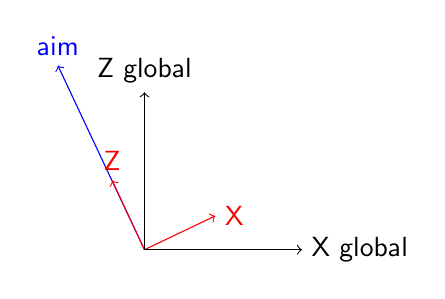
\begin{tikzpicture}
	\draw [->,color=blue] (0,0) -- (-1.1,2.34) node [above] {aim};
	\draw [->,color=red] (0,0) -- (0.9,0.43) node [right] {X};
	\draw [->,color=red] (0,0) -- (-0.41,0.88) node [above] {Z};
	\draw [->] (0,0) -- (2,0) node [right] {X global};
	\draw [->] (0,0) -- (0,2) node [above] {Z global};
\end{tikzpicture}
\caption{Top view of camera's aiming and transform matrix}
\label{fig:camera_aiming}
\end{figure}

\subsection{Projection on a plane based on a normal}
\label{subsec:ortho_projection}
In the chapter \ref{subsec:ground_clamping}, we talk about the velocity that should follow the ground. In chapter \ref{subsec:slopes}, we implement this concept with a mere line of code. In this chapter, I'll explain in a mathematical aspect how we calculate the new velocity.

\paragraph{Dot product}
But first, a little reminder. The dot product of a vector with another vector is the scalar projection (figure \ref{fig:scalar_projection}) of the first vector on the other one. One property of the scalar projection is that the vector to project (here $a$) is the hypotenuse of a right triangle with $c$ as one orthogonal side. And $c$ is oriented like $b$ but with a different length.
\begin{figure}[H]
\centering
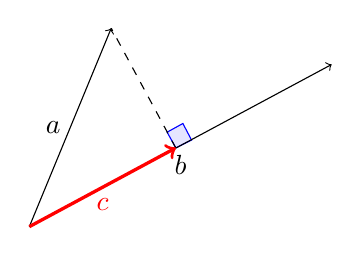
\begin{tikzpicture}
	\draw[color=blue,fill=blue,fill opacity=0.1] (2.06,1.1) -- (1.95,1.31) -- (1.75,1.2) -- (1.86,1) -- cycle; 
	\draw [->] (0,0) -- node[below] {$b$} (3.84,2.06);
	\draw [->] (0,0) -- node[left] {$a$} (1.04,2.52);
	\draw [dash pattern=on 3pt off 3pt] (1.86,1)-- (1.04,2.52);
	\draw [->,line width=1.2pt,color=red] (0,0)-- node[below] {$c$} (1.86,1);
\end{tikzpicture}
\caption{Scalar projection}
\label{fig:scalar_projection}
\end{figure}
In GDScript, there is a vector function called \textit{dot} that returns the length of the projected vector. To get the actual vector like $c$ in the figure, we must multiply the normalized vector $b$ with the dot value, like:
\begin{pythoncode}
  var a=Vector3(...)
  var b=Vector3(...)
  var c = b.dot(a) * b.normalized()
\end{pythoncode}

It is important to notice that the other orthogonal side of the right rectangle is what we're looking for. In figure \ref{fig:wanted_scalar_projection}, the vector we want is $d$ because it's perpendicular to vector $b$.
\begin{figure}[H]
\centering
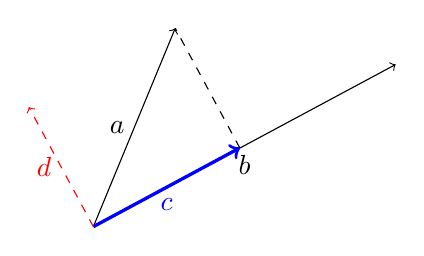
\begin{tikzpicture}
	\draw [->] (0,0) -- node[below] {$b$} (3.84,2.06);
	\draw [->] (0,0) -- node[left] {$a$} (1.04,2.52);
	\draw [dash pattern=on 3pt off 3pt] (1.86,1)-- (1.04,2.52);
	\draw [->,line width=1.2pt,color=blue] (0,0)-- node[below] {$c$} (1.86,1);
	\draw [->,color=red,dash pattern=on 3pt off 3pt] (0,0)-- node[left] {$d$} (-0.82,1.52);

\end{tikzpicture}
\caption{The vector $d$ is perpendicular to vector $b$}
\label{fig:wanted_scalar_projection}
\end{figure}

To obtain vector $d$, we substract the vector $c$ to vector $a$, like in figure \ref{fig:scalar_substraction}
\begin{figure}[H]
\centering
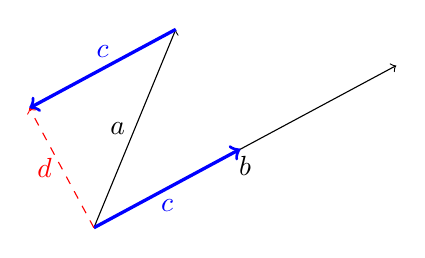
\begin{tikzpicture}
	\draw [->] (0,0) -- node[below] {$b$} (3.84,2.06);
	\draw [->] (0,0) -- node[left] {$a$} (1.04,2.52);
	\draw [->,line width=1.2pt,color=blue] (0,0)-- node[below] {$c$} (1.86,1);
	\draw [->,shift={(-0.82,1.52)},line width=1.2pt,color=blue] (1.86,1)-- node[above] {$c$} (0,0);
	\draw [->,color=red,dash pattern=on 3pt off 3pt] (0,0)-- node[left] {$d$} (-0.82,1.52);
\end{tikzpicture}
\caption{Substraction of the scalar projection}
\label{fig:scalar_substraction}
\end{figure}
In GDScript, the code would be:
\begin{pythoncode}
  var a=Vector3(...)
  var b=Vector3(...)
  var c = b.dot(a) * b.normalized()
  var d = a - c
\end{pythoncode}
And after simplification, it's:
\begin{pythoncode}
  var a=Vector3(...)
  var b=Vector3(...)
  var d = a - b.dot(a) * b.normalized()
\end{pythoncode}

For our tutorial, $a$ is the velocity and $b$ is the normal of the collision, which is by default normalized. And $d$ is the resulting velocity we want to apply to the actor. The final code as implemented is like:
\begin{pythoncode}
  velocity = velocity - normal.dot(velocity) * normal
\end{pythoncode}

You might wonder, why could this work for us since those are 2D vectors and what we use are 3D vectors? What about the 3rd dimension? In fact, it would make no difference if it was 2,3 or 80 dimensions. By using only 2 vectors of our game space, we worked in a non-orthographic 2 dimensions space made from those 2 vectors.

\begin{thebibliography}{1}

\bibitem{github_project} Kinematic FPS demo project\\
https://github.com/gokudomatic/godot

\bibitem{godot} Godot Game Engine {\em Okam Studio} 2014. \\
http://www.godotengine.org/wp/

\bibitem{wiki_godot} Wiki of the Godot Engine\\
Main wiki page : https://github.com/okamstudio/godot/wiki\\
\\
Wiki page about Vectors : https://github.com/okamstudio/godot/wiki/tutorial\_vector\_math\\
Wiki page about quaternions : https://github.com/okamstudio/godot/wiki/tutorial\_transforms

\bibitem{FPSTest} FPS Test demo\\
https://github.com/leezh/godot

\bibitem{blender} Blender\\
http://www.blender.org/

\bibitem{sketchup} Sketchup\\
http://www.sketchup.com/

\bibitem{sketchup_stl} Sketchup STL export script\\
http://www.guitar-list.com/download-software/convert-sketchup-skp-files-dxf-or-stl


\bibitem{fox2d} Fox2d Demo\\
https://github.com/gokudomatic/godot

\bibitem{doom} Doom\\
http://www.idsoftware.com/

\bibitem{freedoom} Freedoom project\\
https://freedoom.github.io/

\end{thebibliography}

\end{document}
